\documentclass[russian]{lecture-notes}

\usepackage[final]{graphicx} % возможность вставлять изображения в текст
\usepackage{subcaption} % пакет нужен, чтобы можно было ставить несколько рисунктов рядом     

\usepackage{amssymb} % для знака пустого множества
\usepackage{amsfonts} % для букв с двойными штрихами (знак натуральных чисел)

\usepackage{tikz}  % для рисования графов
\usetikzlibrary{graphs}
\usepackage{ulem}
\usepackage{pgfplots}

\usepackage{cancel}
\usepackage{amsmath}
\usepackage{textcomp}

\title{Математическая логика и теория алгоритмов}
\lecturer{Поcов Илья Александрович}
\notesauthor{Блюдин Андрей и Хаматов Вадим}

\begin{document}
    \maketitle

    \begin{sloppypar}

        \tableofcontents


        \section{Математическая логика}

        \subsection{Исчисление высказываний}

        \subsubsection{Основные понятия}

        \begin{definition}
            Логическая функция ~--- это множество из 2 элементов. Также, логической функцией называют множество логических значений

            $B = \{0, 1 \}$, где 0 ~--- это ложь (false), а 1 ~--- это истина (true)
        \end{definition}

        \begin{definition}
            Логическая функция от $n$ переменных
            $$f : B^n \rightarrow B$$
        \end{definition}

        \begin{remark}
            Часто логические функции вводят как перечисление возможных аргументов и значений функции при этих аргументах
        \end{remark}

        \begin{example}
            Введем функцию $f(x,y)$

            \begin{table}[h!]
                \centering
                \begin{tabular}{|c|c|c|cl}
                    \cline{1-3}
                    x & y & f(x,y) & & \\ \cline{1-3}
                    0     & 0 & 0      & & \\ \cline{1-3}
                    0     & 1 & 1      & & \\ \cline{1-3}
                    1     & 0 & 1      & & \\ \cline{1-3}
                    1     & 1 & 1      & & \\ \cline{1-3}
                \end{tabular}
                \caption{Таблица истинности для $f(x,y)$}
            \end{table}

            Эту же функцию можно задать функцией $f(x,y) = max(x,y)$
        \end{example}

        \begin{proposition}
            Функция от $n$ переменных может быть $f(x_1, x_2, x_3, \dots, x_n)$

            \begin{table}[h!]
                \centering
                \begin{tabular}{|c|c|c|c|l|}
                    \hline
                    $x_1$ & $x_2$ & ... & $x_n$                  & f($x_1, x_2, \dots, x_n$) \\ \hline
                    0        & 0     & ... & 0                      & 0 или 1                   \\ \hline
                    ...      & ...   & ... & ...                    & 0 или 1                   \\ \hline
                    1        & 1     & ... & \multicolumn{1}{l|}{1} & 0 или 1                   \\ \hline
                \end{tabular}
                \caption{Таблица истинности для $f(x_1,x_2, \dots, x_n)$}
            \end{table}

            При этом количество всех возможных наборов аргументов равняется $2^n$, а количество всех возможных функций при всех возможных наборах аргументов равняется $2^{2^n}$
        \end{proposition}

        \begin{corollary}
            Посчитаем количество таких функий для разных $n$

            $n = 1 \quad 2^2 = 4$ функций $f(x)$

            $n = 2 \quad 2^{2^2} = 16$ функций $f(x,y)$

            $n = 3 \quad 2^{2^3} = 2^8 = 256$ функций $f(x,y,z)$
        \end{corollary}

        \subsubsection{Функции от 1 переменной (их определения)}

        \begin{example}
            Перечислим все возможные функции от 1 переменной

            \begin{table}[h!]
                \centering
                \begin{tabular}{|c|c|c|c|l|}
                    \hline
                    $x$ & $f_1(x)$ & $f_2(x)$ & $f_3(x)$ & $f_4(x)$ \\ \hline
                    0      & 0        & 0        & 1        & 1        \\ \hline
                    1      & 0        & 1        & 0        & 1        \\ \hline
                \end{tabular}
            \end{table}

            Данные функции имеют значение:

            $f_1(x) = 0$ ~--- функция 0

            $f_2(x) = x$ ~--- функция $x$

            $f_3(x) = !x, \bar x, \neg x$, not $x$ ~--- функция отрицания (не $x$)

            $f_4(x) = 1$ ~--- функция 1

        \end{example}

        \subsubsection{Функции от 2 переменных (их определения)}

        \begin{example}
            Перечислим все возможные функции от 2 переменных

            \begin{table}[h!]
                \centering
                \begin{tabular}{|c|c|c|c|c|c|c|c|c|c|}
                    \hline
                    $x$ & $y$ & $f_1(x)$ & $f_2(x)$ & $f_3(x)$ & $f_4(x)$ & $f_5(x)$ & $f_6(x)$ & $f_7(x)$ & $f_8(x)$ \\ \hline
                    0      & 0   & 0        & 0        & 0        & 0        & 0        & 0        & 0        & 0        \\ \hline
                    0      & 1   & 0        & 0        & 0        & 0        & 1        & 1        & 1        & 1        \\ \hline
                    1      & 0   & 0        & 0        & 1        & 1        & 0        & 0        & 1        & 1        \\ \hline
                    1      & 1   & 0        & 1        & 0        & 1        & 0        & 1        & 0        & 1        \\ \hline
                \end{tabular}
                \caption{Таблица истинности для $f(x,y)$}
            \end{table}

            Продолжение:

            \begin{table}[h!]
                \centering
                \begin{tabular}{|c|c|c|c|c|c|c|c|c|c|}
                    \hline
                    $x$ & $y$ & $f_9(x)$ & $f_{10}(x)$ & $f_{11}(x)$ & $f_{12}(x)$ & $f_{13}(x)$ & $f_{14}(x)$ & $f_{15}(x)$ & $f_{16}(x)$ \\ \hline
                    0      & 0   & 1        & 1           & 1           & 1           & 1           & 1           & 1           & 1           \\ \hline
                    0      & 1   & 0        & 0           & 0           & 0           & 1           & 1           & 1           & 1           \\ \hline
                    1      & 0   & 0        & 0           & 1           & 1           & 0           & 0           & 1           & 1           \\ \hline
                    1      & 1   & 0        & 1           & 0           & 1           & 0           & 1           & 0           & 1           \\ \hline
                \end{tabular}
                \caption{Таблица истинности для $f(x,y)$}
            \end{table}

            \textbf{Перечислим основные значения функций:}

            $f_2(x,y)$ ~--- это конъюнкция или "лочическое и"  или логическое умножение ($xy, x\&y, x \wedge y$)

            $f_7(x,y)$ ~--- это исключающее или ($x+y, x XOR y, x \oplus y$), также данную функцию можно ассоциировать как $(x+y) mod 2$

            $f_8(x,y)$ ~--- это логическое или, но ее можно также записать как $max(x,y)$  ($x|y, x \lor y$)

            $f_{10}(x,y)$ ~--- это эквивалентность ($x \Leftrightarrow y, x \equiv y, x == y$)

            $f_{14}(x,y)$ ~--- это импликация ($x \Rightarrow y, x \rightarrow y$)

            Импликация работает так, что истина следует из чего угодно:

            лешия не существует $\Rightarrow$ русалок не существует = 1 (1 $\Rightarrow$ 1 = 1)

            допса скучная $\Rightarrow$ русалок не существует = 1 (0 $\Rightarrow$ 1 = 1)

            русалки существуют $\Rightarrow$ драконы существуют = 1 (0 $\Rightarrow$ 0 = 1)

            x $\Rightarrow$ y = 0 только если x = 1, а y = 0

            $f_{12}(x,y)$ ~--- это обратная импликация ($x \Leftarrow y = y \Rightarrow x$)

            $f_{9}(x,y)$ ~--- стрелка Пирса ($x \downarrow y = \overline{x \lor y}$)

            $f_{15}(x,y)$ ~--- штрих Шеффера ($x | y = \overline{xy}$)

            $f_{3}(x,y)$ ~--- запрет по y ($x > y = \overline{x \Rightarrow y}$)

            $f_{1}(x,y)$ ~--- 0

            $f_{4}(x,y)$ ~--- $x$

            $f_{5}(x,y)$ ~--- запрет по x ($x < y = \overline{x \Leftarrow y}$)

            $f_{6}(x,y)$ ~--- $y$

            $f_{11}(x,y)$ ~--- не y ($\neg y$)

            $f_{13}(x,y)$ ~--- не x ($\neg x$)

            $f_{16}(x,y)$ ~--- 1

        \end{example}

        \begin{definition}
            Логические выражения ~--- способ задания логических функций с помощью переменных, цифр 0 или 1 и операций:

            $\cdot \quad \lor \quad \Rightarrow \quad  \Leftrightarrow \quad + \quad \equiv \quad | \quad \downarrow \quad < \quad >$
        \end{definition}

        \begin{example}
            Примеры логических выражений:

            $(x \lor y) = $

            $(x \Rightarrow yz) \lor (y \equiv z)$

            $(0 \Rightarrow x) \lor (1 \Rightarrow y)$
        \end{example}

        \begin{definition}
            Значения логического выражения можно записать \textbf{Таблицей истинности}
        \end{definition}

        \begin{example}
            $f(x, y, z) = (x \lor y)z$

            \begin{table}[h!]
                \centering
                \begin{tabular}{|c|c|c|c|}
                    \hline
                    x & y & z & f(x,y,z) \\ \hline
                    0    & 0 & 0 & 0        \\ \hline
                    0    & 0 & 1 & 0        \\ \hline
                    0    & 1 & 0 & 0        \\ \hline
                    0    & 1 & 1 & 1        \\ \hline
                    1    & 0 & 0 & 0        \\ \hline
                    1    & 0 & 1 & 1        \\ \hline
                    1    & 1 & 0 & 0        \\ \hline
                    1    & 1 & 1 & 1        \\ \hline
                \end{tabular}
            \end{table}
        \end{example}

        \begin{remark}
            Порядок строчек в таблеце истинности может быть любым, но лучше использовать как у двоичных чисел
        \end{remark}

        \begin{proposition}
            Таблицы истинности часто считают постепенно

            \begin{table}[h!]
                \centering
                \begin{tabular}{|c|c|c|c|l|}
                    \hline
                    x    & y       & z       & $x \lor y$ & $(x \lor y)z$ \\ \hline
                    $\dots$ & $\dots$ & $\dots$ & $\dots$    & $\dots$       \\ \hline
                    $\dots$ & $\dots$ & $\dots$ & $\dots$    & $\dots$       \\ \hline
                \end{tabular}
            \end{table}
        \end{proposition}

        \subsubsection{Приоритеты операций}

        $$\neg$$

        $$\cdot$$

        $$\lor$$

        $$+ \quad \equiv$$

        $$\Rightarrow \quad \Leftarrow$$

        $$| \quad \downarrow \quad < \quad >$$

        \begin{example}
            Примеры приоритетов операций:

            $\neg x \lor y = (\neg x) \lor y$

            $x \lor y z = x \lor (y z)$

            $x \Rightarrow y \lor z = x \Rightarrow (y \lor z)$
        \end{example}

        \subsubsection{Алгебраические преобразования логических выражений}

        \begin{definition}
            Алгебраические преобразования логических выражений ~--- изменяем выражения по правилам, обычно в сторону упрощения
        \end{definition}

        \begin{example}
            $(0 \Rightarrow x) \lor (1 \Rightarrow y) = 1 \lor (1 \Rightarrow y) = 1$
        \end{example}

        \begin{proposition*}
            $$\overline{\overline{x}} = x$$

            \textbf{Доказательство:}

            \begin{table}[h!]
                \centering
                \begin{tabular}{|c|c|c|}
                    \hline
                    $x$ & $\overline{x}$ & $\overline{\overline{x}}$ \\ \hline
                    0      & 1              & 0                         \\ \hline
                    1      & 0              & 1                         \\ \hline
                \end{tabular}
            \end{table}

        \end{proposition*}

        \begin{proposition*}
            При $\lor$:

            $$1 \lor x = 1$$

            $$0 \lor x = x$$

            $$x \lor y = y \lor x$$
        \end{proposition*}

        \subsubsection{Таблица эквивалентных логических выражений}

        \begin{proposition}
            $x \lor y = y \lor x $ - симметричность


            $x \lor 0 = x$


            $x \lor 1 = 1$


            $x \lor x = x$


            $x \lor \overline{x} = 1 $


            $\qquad$ \textbf{Доказательство:}


            \begin{table}[h!]
                \centering
                \begin{tabular}{|c|c|c|}
                    \hline
                    $x$ & $\overline{x}$ & $x \lor \overline{x}$ \\ \hline
                    0      & 1              & $0 \lor 1 = 1$        \\ \hline
                    1      & 0              & $1 \lor 0 = 1$        \\ \hline
                \end{tabular}
            \end{table}

            $xy = yx $

            $x*0 = 0$

            $x*1 = x$

            $x*x = x$

            $x* \overline{x} = 0$

            $x+y = y + x$

            $x + 0 = x$

            $x + 1 = \overline{x}$

            $x + x = 0$

            $x + \overline{x} = 1 $

        \end{proposition}

        \begin{proposition}

            $x \lor (y\lor z) = (x \lor y ) \lor z$ - ассоциативность

            Ассоциативность означает,что порядок скобок не важен

            \begin{example}
                $x \Rightarrow y \neq y \Rightarrow x$ - не симметричная функция

                $$$$

                \textbf{Доказательство: }

                \begin{table}[h!]
                    \centering
                    \begin{tabular}{|l|l|l|}
                        \hline
                        x y & $x \Rightarrow y$ & $y \Rightarrow x$ \\ \hline
                        0 0 & 1                 & 1                 \\ \hline
                        0 1 & 1                 & 0                 \\ \hline
                        1 0 & 0                 & 1                 \\ \hline
                        1 1 & 1                 & 1                 \\ \hline
                    \end{tabular}
                \end{table}

            \end{example}

            \begin{remark}
                $x \Rightarrow y \neq y\Rightarrow x$
            \end{remark}

            $x \Rightarrow 0 = \overline{x}$

            $0 \Rightarrow x = 1$
            $$$$

            \textbf{Доказательство: }

            \begin{table}[h!]
                \centering
                \begin{tabular}{|l|l|}
                    \hline
                    x & $x \Rightarrow 0$     \\ \hline
                    0 & $0 \Rightarrow 0 = 1$ \\ \hline
                    1 & $1 \Rightarrow 0 = 0$ \\ \hline
                \end{tabular}
            \end{table}

            $x\Rightarrow 1 = 1$

            $1 \Rightarrow x = x$

            $x \Rightarrow x = 1$

            $x \Rightarrow \overline{x} = \overline{x}$

            $\overline{x} \Rightarrow x = x$

            $\overline{x} \Rightarrow y \Rightarrow z$ договоримся, что это $x \Rightarrow y (y\Rightarrow z) \neq (x \Rightarrow y) \Rightarrow z$

            \begin{table}[h!]
                \centering
                \begin{tabular}{|l|l|l|l|l|}
                    \hline
                    x y z & $x \Rightarrow y$ & $y \Rightarrow z$ & $x \Rightarrow (y \Rightarrow z)$ & $(x \Rightarrow y) \Rightarrow z$ \\ \hline
                    0 0 0  & 1                 & 1                 & 1                                 & 0                                 \\ \hline
                    0 0 1 & 1                 & 1                 & 1                                 & 1                                 \\ \hline
                    0 1 0 & 1                 & 0                 & 1                                 & 0                                 \\ \hline
                    0 1 1 & 1                 & 1                 & 1                                 & 1                                 \\ \hline
                    1 0 0 & 0                 & 1                 & 1                                 & 1                                 \\ \hline
                    1 0 1 & 0                 & 1                 & 1                                 & 1                                 \\ \hline
                    1 1 0 & 1                 & 0                 & 0                                 & 0                                 \\ \hline
                    1 1 1 & 1                 & 1                 & 1                                 & 1                                 \\ \hline
                \end{tabular}
            \end{table}

            $x \Leftrightarrow y = y \Leftrightarrow x$

            $x \Leftrightarrow 0 = \overline{x}$

            $x \Leftrightarrow 1 = x$

            $x \Leftrightarrow x =1$

            $x \Leftrightarrow \overline{x} = 0$

            $x \Leftrightarrow (y\Leftrightarrow z) = (x \Leftrightarrow y) \Leftrightarrow z$ - ассоциативно

        \end{proposition}

        \begin{proposition}

            Дистрибутивность

            $(x \lor y) z = xz \lor yz$

            $(x+y)z = xz + yz$ по таблице истинности

            $(x \& y ) \lor z$ ($xy \lor z = (x \lor z)(y \lor z)$

            $(x \lor y) \& z = (x \& z) \lor (y \& z)$

            $(x \& y) \lor z = (x \lor z) \& (y\lor z)$

            \begin{remark}

                $ $
                $(x_{1} \lor x_{2} \lor x_{3}) (y_{1} \lor y_{2}) = (x_{1} \lor x_{2} \lor x_{3})y_{1} \lor (x_{1} \lor x_{2} \lor x_{3})y_{2} = x_{1}y_{1} \lor x_{2}y_{1} \lor x_{3}y_{1} \lor x_{1}y_{2} \lor x_{2}y_{2} \lor x_{3}y_{2}$

                $xy \lor z = (x \lor z)(y\lor z) = xy \lor xz \lor zy \lor zz = xy \lor  xz \lor zy \lor z = xy \lor xz \lor zy \lor z*1 = xy \lor z(x\lor y \lor 1) = xy \lor z$ сошлось

            \end{remark}

            $x+y = \overline{x\Rightarrow}y$ - смотри Таблицу истинности

            $(x\Rightarrow y)(y\Rightarrow x) = x \Rightarrow y$

            \subsubsection{Многочлены Жегалкина}

            \begin{remark}

                Одну и ту же функцию можно записать по разному.

            \end{remark}

            В алгебре: $f(x) = 1 +x = x + 1 = x + 5 - 4 = sin(x-x) + x = ...$

            В логике: $f(x,y) = x \lor y = x \lor y \lor 0 = (x \lor y)(\overline{y} \lor y = x\overline{y} \lor y$ (= - дистрибутивность)

            \textbf{Многочлены Жегалкина для логической формулы}


            \begin{definition}
                $f(x_{1}......x_{n}$) - это многочлен с переменными xi, конспектами 0,1 и со степенями переменных $\leqslant$ 1. Это многочлены от xi $\mathbf{Z_{2}}$
            \end{definition}

            \begin{example}

                $f(x,y,z) = 1 + x + yz + xyz$

                $1 + x \qquad \qquad xy+xyz$

                $1 + xy$
            \end{example}

            Не многочлены

            $1 + x + (y \lor z)$

            $1 + x + z^{2}$ нельзя степень 2


            \begin{remark}
                В общем случае многочлен от 1 переменной ($a_{i} =$ 0 или 1)

                $a_{0} + a_{1}x$

                от 2ух: $a_{0} + a_{1}x+a{2}y+a{3}xy$

                от 3ех: $a_{0} + a_{1}x + a_{2}y + a_{3}z + a_{4}xy + a_{5}xz + a_{6}yz + a_{7}xyz$

            \end{remark}

            В общем случае $f(x1....x_{n}$) $a_{0} + a_{1}x_{1} + ... + a_{n}x_{n} + ax_{1}x_{2} + ax_{1}x_{3}$ + ... (все пары переменных) + $ ax_{1}x_{2}x_{3}+ax_{1}x_{3}x_{2} \leftarrow $все тройки перменных$ + ax_{1}x_{2}x_{3}...x_{n}$

            \begin{definition}
                $\forall f(x_{1}...x_{n})$ - логические функция $\exists!$ многочлен Жегалкина $g(x_{1}...x_{n}) : f = g$
            \end{definition}

            \begin{remark}
                Всего 4 функции от 1ой переменной

                $f(x) = 0 = \overline{x} = 0 + 0x$

                $f(x) = 1 = 1 = 1 + 0x$

                $f(x) = x = x = 0 + 1x$

                $f(x) = \overline{x} = 1 + x = 1 + 1x$
            \end{remark}

            \textbf{Доказательство:}

            \begin{definition}
                Разные многочлены - это разные логические функции т.е. $f(x_{1} ... x_{n} = a_{0} + ... + a_{1}x_{1} ... x_{n}$

                $g(x_{1}...x_{n}) = b_{0} + ... + bx_{1} ... x_{n}$

                $\exists!$ : $a_{i} \neq b_{i}$ различающийся

            \end{definition}

            \qquad \textbf{Доказательство:}

            Возьмем индекс с самым большик количеством переменных

            $f(x,y,z) = 1 + x + xy + xyz = ... + 1x + Dy + Dz + 1xy$

            $g(x,y,z) = 1 + y + z + xyz ... + Dx + 1y + 1z$

            для переменных этого слагаемого подставим 1 0xy

            для остальных переменных : 0

            [ В примере $x=1,y=0,z=0 : f(1,0,0)$ и $g(1,0,0)$ ]

            и в f и в g все другие слагаемые равны 0

            Теперь f(...) и g(...)

            $f(...) = a_{i}x{1}x_{2}x_{3} \neq b_{i}x_{1}x_{2}x_{3}$ $\Rightarrow f(x_{1}...x_{n}$) $\neq y$

            \qquad \textbf{Доказательство:}

            Проверим, что многочленов Жегалкина столько, сколько функций:

            Посчитаем

            $a_{0} + a_{1}x_{1}+ ... + a_{1}x_{1}x_{2}...x_{n}$

            Сколько слагаемых:

            1) 1 слагаемых без переменных

            n слагаемых с переменной

            \qquad $a_{1}x_{1} + ... + a_{n}x_{n}$

            $C_{n}^{2}$ - слагаемых с 2 - мя переменными

            $C_{n}^{3}$ - слагаемых с 3 - мя переменными

            $C_{n}^{n}$ - слагаемых с n переменными

            Всего : $ C_{n}^{0} + C_{n}^{1} + C_{n}^{2} + ... C_{n}^{n} = 2^{n}((1+1)^{2}) $

            \begin{example}

                $a_{0} + a_{1}x$ - 2 слагаемых

                $a_{0} + a_{1}x + a_{2}y+a_{3}xy - 2^2 = 4$ слагаемых

                2) Все слагаемых имею вид: $x_{1},x_{2},x_{3}...x_{n}$ (0 или 1) - $2^n$ слагаемых

                Итого: многочлен Жегалкина от n переменных
            \end{example}


            \begin{problem}
                Сколько разных многочленов?

                Это столько же, сколько логический функций

                Итог:

                \textbf{Следствие:} Любая логическая функция может быть представлена в виде многочлена Жегалкина

            \end{problem}

            \begin{example}

                $f(x,y) = x \lor y$

                $f(x,y) = x*y$ - уже многочлен Жегалкина

                \textbf{Метод неопределенных коэффициентов:}


                Подберем $x \lor y = a_{0} + a_{1}x + a_{2}y + a_{3}xy$

                $f(0,0) = 0$

                $f(0,0) = a_{0} + a_{1}*0 + a_{2}*0 + a_{3}...$

                $f(1,0) = 1 \lor 0 = 1$

                $f(1,0) = a_{0} + a_{1} = a_{1}$ ($a_{0} = 0, \Rightarrow a_{1} = 1$

                $f(0,1) =$ аналогично $\Rightarrow a_{1} = 1$

                $f(x,y) = x+y + a_{3}xy$

                $f(1,1) = 1 \lor 1 = 1$

                $f(1,1) = 1 + 1 + a_{3} = 0 + a_{3} = a_{3}$, $a_{3}=1$

                Ответ: $x\lor y = x+y+xy$

            \end{example}

        \end{proposition}

        \textbf{Многочлены Жегалкина от 1 переменной:}

        \begin{table}[h!]
            \centering
            \begin{tabular}{|c|c|}
                \hline
                $f(x)$  & Мн Ж    \\ \hline
                0       & 0       \\ \hline
                1       & 1       \\ \hline
                $x$       & $x$     \\ \hline
                $\bar{x}$ & $1 + x$ \\ \hline
            \end{tabular}
        \end{table}

        \textbf{Многочлены Жегалкина от 2 переменных:}

        \begin{table}[h!]
            \centering
            \begin{tabular}{|c|c|}
                \hline
                $f(x)$   & Мн Ж         \\ \hline
                0        & 0            \\ \hline
                1        & 1            \\ \hline
                $xy$       & $xy$         \\ \hline
                $x + y$    & $x + y$      \\ \hline
                $x \lor y$ & $x + y + xy$ \\ \hline
            \end{tabular}
        \end{table}

        \textbf{Формулы:}

        \begin{enumerate}
            \item    $\overline{xy} = \neg (xy) = \overline{x} \lor \overline{y} $
            \item $\overline{x \lor y} = \neg (x \lor y) = \overline{x} \cdot \overline{y} = \overline{x} \: \overline{y}$
        \end{enumerate}

        \begin{remark}
            $\overline{xy} \neq \overline{x} \cdot \overline{y} = \overline{x} \: \overline{y}$
        \end{remark}

        \textbf{Доказательство формул через таблицу истинности:}

        \begin{table}[h!]
            \centering
            \begin{tabular}{|c|c|c|c|}
                \hline
                $x$ & $y$ & $\overline{x \lor y}$ & $\overline{x} \cdot \overline{y}$ \\ \hline
                0     & 0   & 1                     & 1                                 \\ \hline
                0     & 1   & 0                     & 0                                 \\ \hline
                1     & 0   & 0                     & 0                                 \\ \hline
                1     & 1   & 0                     & 0                                 \\ \hline
            \end{tabular}
        \end{table}

        \subsubsection{Получение многочлена Жегалкина через алгебраические упрощения}

        \begin{enumerate}
            \item{
                \textbf{Многочлен Жегалкина для $\lor$}

                $x \lor y = (x = \overline{a}, y = \overline{y}) = \overline{ab} = \overline{\overline{x} \cdot \overline{y}} = \overline{(1 + x)(1 + y)} = 1 + (1 + x)(1 + y) = 1 + 1 + x + y + xy = \underline{x + y + xy}$
            }

            \item{
                \textbf{Многочлен Жегалкина для $\Leftrightarrow$}

                $x \Leftrightarrow y = \overline{x + y} = \underline{1 + x + y}$
            }

            \item{
                \textbf{Многочлен Жегалкина для $\Rightarrow$}

                $x \Rightarrow y = \overline{x} \lor y = (1 + x) \lor y = (1 + x) + y + (1 + x)y = 1 + x + y + y + xy = \underline{1 + x + xy}$
            }
        \end{enumerate}

        \begin{remark}

            Если есть логическая формула, то ее можно приветси к форме многочлена Жегалкина двумя способами:

            \begin{enumerate}
                \item{
                    метод неопределенных коэффициентов:

                    $a_0 + a_1x + a_2y + a_3z + \dots + axyz$
                }
                \item{
                    метод алгебраических преобразований
                }
            \end{enumerate}

            \begin{example}
                $x \lor y = \overline{\overline{x} \cdot \overline{y}} = \dots = x + y + xy$
            \end{example}

            \begin{example}
                $x \Rightarrow y = \overline{x} \lor y = \dots = 1 + x + xy$
            \end{example}

            \begin{example}
                $x \Rightarrow (y \lor \overline{z}) = x \Rightarrow (y + \overline{z} + y \cdot \overline{z}) = x \Rightarrow (y + (1 + z) + y \cdot (1 + z))  = x \Rightarrow (y + 1 + z + y + yz) = x \Rightarrow (1 + z + yz) = 1 + x + x(1 + z + yz) = 1 + x + x + xz + xyz = 1 + xz + xyz $
            \end{example}

        \end{remark}

        \textbf{Поймем, что:}
        $(x \Leftrightarrow y) \Leftrightarrow z = x \Leftrightarrow (y \Leftrightarrow z)$

        $x \Leftrightarrow y \Leftrightarrow z = (1 + x + y) \Leftrightarrow z = 1 + (1 + x + y) + z  = 1 + 1 + x + y + z = x + y + z $

        \textbf{Вывод:}

        Заранее не ясно, сложно ли привести логическую формулу к многочлену Жегалкина

        \subsubsection{Дизъюнктивно-нормальная форма (ДНФ)}

        \begin{definition}
            Литерал ~--- это переменная или отрицание переменной
        \end{definition}

        \begin{example}
            $x, \overline{x}, y, \overline{y}, z, \overline{z}$
        \end{example}

        \begin{definition}
            Конъюнктор ~--- конъюнкция литералов
        \end{definition}

        \begin{example}
            $x\overline{y}, xyz, \overline{x} \: \overline{y} \: \overline{z}, \overline{x}z,$ ноль (пустой конъюнкт).
        \end{example}

        \begin{definition}
            Логическое выражение имеет ДНФ, если она является дизъюнкцией конъюнкторов
        \end{definition}

        \begin{example}
            $x\overline{y} \lor \overline{x} \: \overline{z} \lor z \lor \overline{x} \: \overline{y}$ ~--- ДНФ
        \end{example}

        \begin{example}
            $xy \lor \overline{x} \: \overline{y}$ ~--- ДНФ
        \end{example}

        \begin{example}
            $x \lor y$ ~--- ДНФ
        \end{example}

        \begin{example}
            $xy$ ~--- ДНФ
        \end{example}

        \begin{example}
            не ДНФ ~--- $\overline{xy} = \overline{x} \lor \overline{y}$ ~---  ДНФ
        \end{example}

        \begin{example}
            не ДНФ ~--- $x \Rightarrow yz = \overline{x} \lor yz$ ~---  ДНФ
        \end{example}

        \textbf{Построение ДНФ по таблице истинности функции:}

        алгоритм на примере трех переменных

        \begin{table}[h!]
            \centering
            \begin{tabular}{|c|c|c|c|c|}
                \hline
                $x$ & $y$ & $z$ & $f(x, y ,z)$ &                                     \\ \hline
                0     & 0   & 0   & 0            &                                     \\ \hline
                0     & 0   & 1   & 0            &                                     \\ \hline
                0     & 1   & 0   & 1            & $\overline{x} \: y \: \overline{z}$ \\ \hline
                0     & 1   & 1   & 1            & $\overline{x} \: yz$                \\ \hline
                1     & 0   & 0   & 0            &                                     \\ \hline
                1     & 0   & 1   & 0            &                                     \\ \hline
                1     & 1   & 0   & 1            & $xy \: \overline{z}$                \\ \hline
                1     & 1   & 1   & 0            &                                     \\ \hline
            \end{tabular}
        \end{table}

        Берем строки из столбца $f(x, y, z)$, где значения в столбце равны 1

        Допустим есть строка: $x = a_1, y = a_2, z = a_3$ ($a$ могут быть как 0, так и 1)

        В ответ добавляется конъюнкт $xyz$ (0 $\Rightarrow$ отрицание, 1 $\Rightarrow$ не отрицание)

        Ответ: $f(x, y, z) = \overline{x} \: y \: \overline{z} \lor \overline{x} \: yz \lor xy \: \overline{z}$

        \textbf{Доказательство корректности алгоритма:}

        Когда полученный ДНФ = 1?

        Когда есть конъюнкт равный 1

        \begin{enumerate}
            \item{
                Если первый конъюнкт равняется 1 (в примере    $\overline{x} \: y \: \overline{z}  = 1)$

                $\Rightarrow $ все литералы конъюнкта равняются 1

                $\Rightarrow$ в примере $\overline{x} = 1 \quad y = 1 \quad \overline{z} = 1$

                $ \qquad \qquad \qquad x = 0 \quad y = 1 \quad z = 0$
            }
            \item{
                Если второй конъюнкт равняется 1

                $\Rightarrow$ в примере $x = 0 \quad y = 1 \quad z = 1$ ~--- строка из таблицы истинности
            }
            \item{
                То же самое с третьим конъюнктом
            }
        \end{enumerate}

        Посмотрим таблицу с этими конъюнктами:

        \begin{table}[h!]
            \centering
            \begin{tabular}{|c|c|c|c|c|c|c|}
                \hline
                $x$ & $y$ & $z$ & $\overline{x} \: y \: \overline{z}$ & $\overline{x} \: yz$ & $xy \: \overline{z}$ & $f(x, y, z)$ \\ \hline
                0     & 0   & 0   & 0                                   & 0                    & 0                    & 0            \\ \hline
                0     & 0   & 1   & 0                                   & 0                    & 0                    & 0            \\ \hline
                0     & 1   & 0   & 1                                   & 0                    & 0                    & 1            \\ \hline
                0     & 1   & 1   & 0                                   & 1                    & 0                    & 1            \\ \hline
                1     & 0   & 0   & 0                                   & 0                    & 0                    & 0            \\ \hline
                1     & 0   & 1   & 0                                   & 0                    & 0                    & 0            \\ \hline
                1     & 1   & 0   & 0                                   & 0                    & 1                    & 1            \\ \hline
                1     & 1   & 1   & 0                                   & 0                    & 0                    & 0            \\ \hline
            \end{tabular}
        \end{table}

        \begin{remark}
            У одной функции могут быть разные ДНФ
        \end{remark}

        \begin{example}
            $\underline{\overline{x} \: y \: \overline{z} \lor \overline{x} \: yz \lor xy \: \overline{z}} = \overline{x} \: y (\overline{z} \lor z) \lor xy \: \overline{z} = \underline{\overline{x} \: y \lor xy \: \overline{z}}$ ~--- подчеркнутые выражения являются ДНФ
        \end{example}

        \begin{example}
            $\underline{\overline{x} \: y \: \overline{z} \lor \overline{x} \: yz \lor xy \: \overline{z}} = \overline{z} \: y (\overline{x} \lor x) \lor zy \: \overline{x} = \underline{\overline{z} \: y \lor zy \: \overline{x}} = \underline{y \: \overline{z} \lor \overline{x} \: yz \lor \overline{x} \: x \lor z \: \overline{z}}$ ~--- подчеркнутые выражения являются ДНФ
        \end{example}

        Получить ДНФ для логической функции/формулы можно:
        \begin{enumerate}
            \item по таблице истинности
            \item с помощью алгебраических преобразований
        \end{enumerate}

        \begin{example}
            \begin{enumerate}
                \item $\overline{x} = \overline{x}$
                \item $x \lor y = x \lor y$
                \item $x \cdot y = x \cdot y$
                \item $x \Rightarrow y = \overline{x} \lor y$
                \item $x \Leftrightarrow y = (x \Rightarrow y)(y \Rightarrow x) = (\overline{x} \lor y)(\overline{y} \lor x) = \overline{x} \: \overline{y} \lor \overline{x} \: x \lor y \: \overline{y} \lor yx = \overline{x} \: \overline{y} \lor xy $

                \begin{table}[h!]
                    \centering
                    \begin{tabular}{|c|c|c|}
                        \hline
                        $x$ & $y$ & $x \Leftrightarrow y$ \\ \hline
                        0       & 0   & 1                     \\ \hline
                        0       & 1   & 0                     \\ \hline
                        1       & 0   & 0                     \\ \hline
                        1       & 1   & 1                     \\ \hline
                    \end{tabular}
                \end{table}

                \item{ $x + y = \overline{x \Leftrightarrow y} = \overline{\overline{x} \: \overline{y} \lor xy} \dots$

                    $ = \overline{\overline{x} \: y} \lor \overline{x \lor \overline{y}} = \overline{\overline{x}} \cdot \overline{y} \lor \overline{x} \cdot \overline{\overline{y}} = x \: \overline{y} \lor \overline{x} \: y$
                }
                \item $x \Rightarrow (y + z) = \overline{x} \lor (y + z) = \overline{x} \lor \overline{y} \: z \lor y \: \overline{z}$
            \end{enumerate}
        \end{example}

        \subsubsection{Задача (не) выполнимости}

        Дана логическая формала в ДНФ

        Проверить, бывает ли она равна 0?

        $\overline{x} \: \overline{y} \lor x \lor y ?= 0$

        $x = 0, y = 0 \Rightarrow \overline{x} \: \overline{y} = 1$

        $\Rightarrow$ данный ДНФ не может быть равным 0

        Эта задача обладает особенностью:

        \begin{enumerate}
            \item если знать значения переменных (ответ), то их легко можно быстро проверить
            \item подобрать значения переменных для 0 ~--- нет
        \end{enumerate}

        Нет известного алгоритма, который "принципиально" быстрее полного перебора

        У этой задачи класс NP выполнимости (ответ легко проверить, а найти его простым способом невозможно)

        \begin{corollary}
            То к чему сводится задача (не) выполнимости тоже сложна
            \begin{enumerate}
                \item упростить логическое выражение
                \item поиск минимального ДНФ
            \end{enumerate}
        \end{corollary}

        \subsubsection{Запись таблиц истинности в виде графика}

        Формула  = $f(x, y, z) = x + y$

        $$f(0, 0) = 0$$

        $$f(0, 1) = 1$$

        $$f(1, 0) = 1$$

        $$f(1, 1) = 0$$

        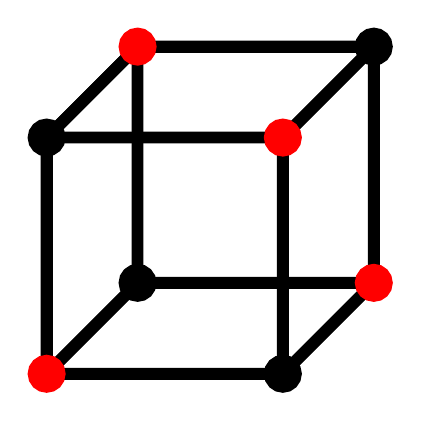
\begin{tikzpicture}[scale=3,line width=1.5mm]

            \draw [circle] (1,0,0) -- (1,0,1) -- (1,1,1) -- (1,1,0) -- cycle;
            \draw [circle] (0,0,0) -- (0,0,1) -- (0,1,1) -- (0,1,0) -- cycle;

            \draw [circle] (0,0,0)   -- (1,0,0)  -- (1,0,1)  -- (0,0,1)  -- cycle;
            \draw [circle] (0,1,0)   -- (1,1,0)  -- (1,1,1)  -- (0,1,1)  -- cycle;

            \draw [circle] (0,0,0)  node[draw, fill = black] (nodeA) {}  -- (1,0,0)  node[draw, fill = red, red] (nodeA) {}  -- (1,1,0)  node[draw, fill = black] (nodeA) {}  -- (0,1,0)  node[draw, fill = red, red] (nodeA) {}  -- cycle;
            \draw [circle] (0,0,1)  node[draw, fill = red, red] (nodeA) {}  -- (1,0,1)  node[draw, fill = black] (nodeA) {}  -- (1,1,1)  node[draw, fill = red, red] (nodeA) {}  -- (0,1,1)  node[draw, fill = black] (nodeA) {}  -- cycle;

        \end{tikzpicture}

        \subsubsection{Задача минимизации ДНФ}

        Данная задача тоже является сложной, также как и задача (не) выполнимости

        Дана логическая функция (в виде ДНФ). Необходимо найти самую короткую ДНФ эквивалентную данной.

        Минимальной ДНФ считается та, где меньше количество литералов и дизъюнкций

        \begin{example}
            $\overline{x} \: \overline{y} \lor z$ короче, чем $xy \lor yz$
        \end{example}

        \begin{remark}
            Далее рассматриваться все будет для функции от 3 переменных $f(x, y, z)$
        \end{remark}

        \begin{remark}
            Какова таблица истинности $xyz = abc$, где $a = 0$ или $1, b = 0$ и $1, c = 0$ или $1$

            $0 \Rightarrow$ надо поставить отрицание

            $1 \Rightarrow$ нет отрицания
        \end{remark}

        \begin{example}
            $f(x, y, z) = \overline{x} \: y \: \overline{z}$

            Если $\overline{x} \: y \: \overline{z} = 1$

            $\Rightarrow \overline{x} = 1,  y = 1, \overline{z} = 1$

            $\Rightarrow x = 0,  y = 1, z = 0$

            $\Rightarrow x = a, y = b, z = c$

            $\Rightarrow a = 0, b = 1, c = 0$

            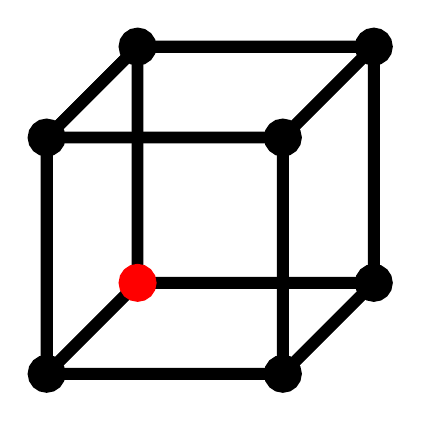
\begin{tikzpicture}[scale=3,line width=1.5mm]

                \draw [circle] (1,0,0) -- (1,0,1) -- (1,1,1) -- (1,1,0) -- cycle;
                \draw [circle] (0,0,0) -- (0,0,1) -- (0,1,1) -- (0,1,0) -- cycle;

                \draw [circle] (0,0,0)   -- (1,0,0)  -- (1,0,1)  -- (0,0,1)  -- cycle;
                \draw [circle] (0,1,0)   -- (1,1,0)  -- (1,1,1)  -- (0,1,1)  -- cycle;

                \draw [circle] (0,0,0)  node[draw, fill = red, red] (nodeA) {}  -- (1,0,0)  node[draw, fill = black] (nodeA) {}  -- (1,1,0)  node[draw, fill = black] (nodeA) {}  -- (0,1,0)  node[draw, fill = black] (nodeA) {}  -- cycle;
                \draw [circle] (0,0,1)  node[draw, fill = black] (nodeA) {}  -- (1,0,1)  node[draw, fill = black] (nodeA) {}  -- (1,1,1)  node[draw, fill = black] (nodeA) {}  -- (0,1,1)  node[draw, fill = black] (nodeA) {}  -- cycle;

            \end{tikzpicture}

        \end{example}



        \begin{example}
            $f(x, y, z) = xy$

            Если $xy = 1$

            $\Rightarrow x = 1,  y = 1$

            $\Rightarrow x = a, y = b$

            $\Rightarrow a = 1, b = 1$

            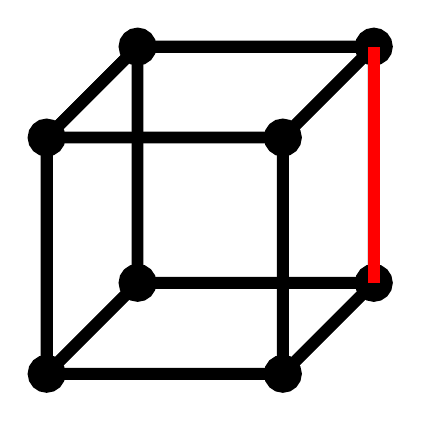
\begin{tikzpicture}[scale=3,line width=1.5mm]

                \draw [circle] (1,0,0) -- (1,0,1) -- (1,1,1) -- (1,1,0) -- cycle;
                \draw [circle] (0,0,0) -- (0,0,1) -- (0,1,1) -- (0,1,0) -- cycle;

                \draw [circle] (0,0,0)   -- (1,0,0)  -- (1,0,1)  -- (0,0,1)  -- cycle;
                \draw [circle] (0,1,0)   -- (1,1,0)  -- (1,1,1)  -- (0,1,1)  -- cycle;

                \draw [circle] (0,0,0)  node[draw, fill = black] (nodeA) {}  -- (1,0,0)  node[draw, fill = black] (nodeA) {}  -- (1,1,0)  node[draw, fill = black] (nodeA) {}  -- (0,1,0)  node[draw, fill = black] (nodeA) {}  -- cycle;
                \draw [circle] (0,0,1)  node[draw, fill = black] (nodeA) {}  -- (1,0,1)  node[draw, fill = black] (nodeA) {}  -- (1,1,1)  node[draw, fill = black] (nodeA) {}  -- (0,1,1)  node[draw, fill = black] (nodeA) {}  -- cycle;

                \draw [red] (1,0,0) -- (1,1,0);

            \end{tikzpicture}

            Аналогично, $f(x, y, z) = \overline{y} \: \overline{z}$

            ребро: $y = 0, z = 0, x = ?$ ~--- не важно

            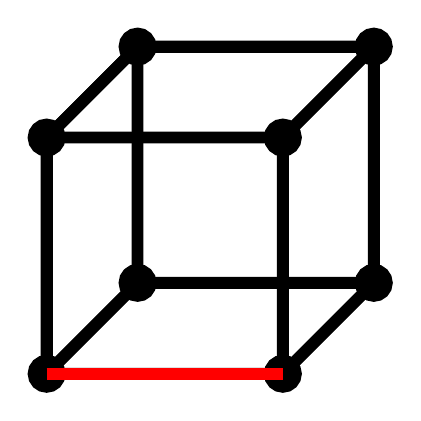
\begin{tikzpicture}[scale=3,line width=1.5mm]

                \draw [circle] (1,0,0) -- (1,0,1) -- (1,1,1) -- (1,1,0) -- cycle;
                \draw [circle] (0,0,0) -- (0,0,1) -- (0,1,1) -- (0,1,0) -- cycle;

                \draw [circle] (0,0,0)   -- (1,0,0)  -- (1,0,1)  -- (0,0,1)  -- cycle;
                \draw [circle] (0,1,0)   -- (1,1,0)  -- (1,1,1)  -- (0,1,1)  -- cycle;

                \draw [circle] (0,0,0)  node[draw, fill = black] (nodeA) {}  -- (1,0,0)  node[draw, fill = black] (nodeA) {}  -- (1,1,0)  node[draw, fill = black] (nodeA) {}  -- (0,1,0)  node[draw, fill = black] (nodeA) {}  -- cycle;
                \draw [circle] (0,0,1)  node[draw, fill = black] (nodeA) {}  -- (1,0,1)  node[draw, fill = black] (nodeA) {}  -- (1,1,1)  node[draw, fill = black] (nodeA) {}  -- (0,1,1)  node[draw, fill = black] (nodeA) {}  -- cycle;

                \draw [red] (0,0,1) -- (1,0,1);

            \end{tikzpicture}

        \end{example}

        Последнее ~--- конъюнкт из 1 литерала:

        $x, \overline{x}, y, \overline{y}, z, \overline{z}$

        \begin{example}

            $f(x, y, z) = \overline{y}$

            Если $\overline{y} = 1$

            $\Rightarrow y = 0, x = ?, z = ?$

            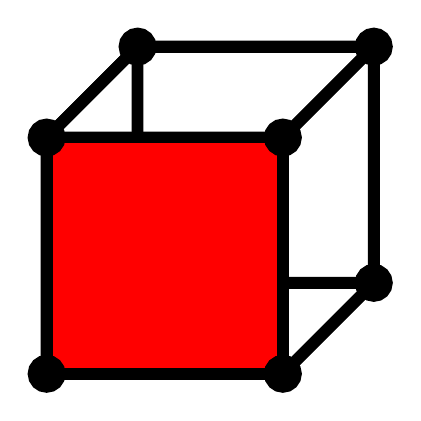
\begin{tikzpicture}[scale=3,line width=1.5mm]

                \draw [circle] (1,0,0) -- (1,0,1) -- (1,1,1) -- (1,1,0) -- cycle;
                \draw [circle] (0,0,0) -- (0,0,1) -- (0,1,1) -- (0,1,0) -- cycle;

                \draw [circle] (0,0,0)   -- (1,0,0)  -- (1,0,1)  -- (0,0,1)  -- cycle;
                \draw [circle] (0,1,0)   -- (1,1,0)  -- (1,1,1)  -- (0,1,1)  -- cycle;

                \draw [circle] (0,0,0)  node[draw, fill = black] (nodeA) {}  -- (1,0,0)  node[draw, fill = black] (nodeA) {}  -- (1,1,0)  node[draw, fill = black] (nodeA) {}  -- (0,1,0)  node[draw, fill = black] (nodeA) {}  -- cycle;
                \draw [circle, fill = red] (0,0,1)  node[draw, fill = black] (nodeA) {}  -- (1,0,1)  node[draw, fill = black] (nodeA) {}  -- (1,1,1)  node[draw, fill = black] (nodeA) {}  -- (0,1,1)  node[draw, fill = black] (nodeA) {}  -- cycle;

            \end{tikzpicture}

            Или конъюнкт $x$, грань $x = 1$

            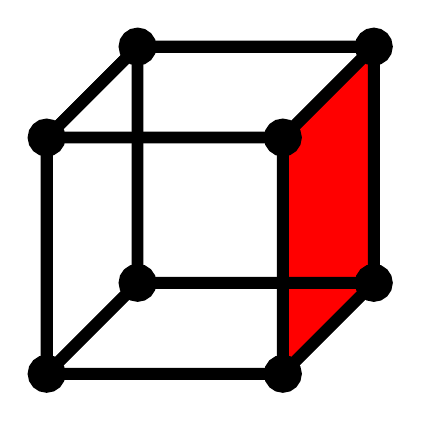
\begin{tikzpicture}[scale=3,line width=1.5mm]

                \draw [circle, fill = red] (1,0,0) -- (1,0,1) -- (1,1,1) -- (1,1,0) -- cycle;
                \draw [circle] (0,0,0) -- (0,0,1) -- (0,1,1) -- (0,1,0) -- cycle;

                \draw [circle] (0,0,0)   -- (1,0,0)  -- (1,0,1)  -- (0,0,1)  -- cycle;
                \draw [circle] (0,1,0)   -- (1,1,0)  -- (1,1,1)  -- (0,1,1)  -- cycle;

                \draw [circle] (0,0,0)  node[draw, fill = black] (nodeA) {}  -- (1,0,0)  node[draw, fill = black] (nodeA) {}  -- (1,1,0)  node[draw, fill = black] (nodeA) {}  -- (0,1,0)  node[draw, fill = black] (nodeA) {}  -- cycle;
                \draw [circle] (0,0,1)  node[draw, fill = black] (nodeA) {}  -- (1,0,1)  node[draw, fill = black] (nodeA) {}  -- (1,1,1)  node[draw, fill = black] (nodeA) {}  -- (0,1,1)  node[draw, fill = black] (nodeA) {}  -- cycle;

            \end{tikzpicture}

        \end{example}

        \textbf{Итого:}

        $xyz$ ~--- это вершина $x = a, y = b, z = c$

        $xy$ ~--- это ребро $x = a, y = b$

        $x$ ~--- это грань $x = a$

        \textbf{Попробуем минимизировать ДНФ}

        \begin{example}

            $\overline{x} \: \overline{y} \: \overline{z} \lor x \: \overline{y} \: \overline{z} \lor xy \: \overline{z}$

            Найти самый короткий ДНФ для данного выражения

            \textbf{Шаг 1: строим ТИ}

            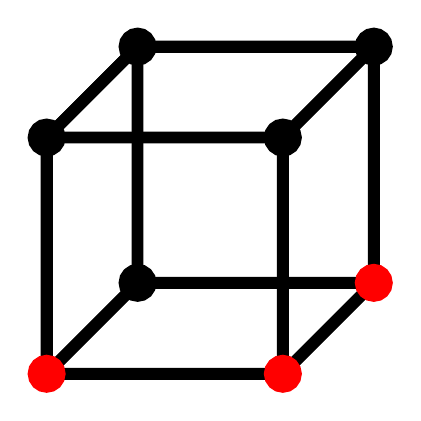
\begin{tikzpicture}[scale=3,line width=1.5mm]

                \draw [circle] (1,0,0) -- (1,0,1) -- (1,1,1) -- (1,1,0) -- cycle;
                \draw [circle] (0,0,0) -- (0,0,1) -- (0,1,1) -- (0,1,0) -- cycle;

                \draw [circle] (0,0,0)   -- (1,0,0)  -- (1,0,1)  -- (0,0,1)  -- cycle;
                \draw [circle] (0,1,0)   -- (1,1,0)  -- (1,1,1)  -- (0,1,1)  -- cycle;

                \draw [circle] (0,0,0)  node[draw, fill = black] (nodeA) {}  -- (1,0,0)  node[draw, fill = red, red] (nodeA) {}  -- (1,1,0)  node[draw, fill = black] (nodeA) {}  -- (0,1,0)  node[draw, fill = black] (nodeA) {}  -- cycle;
                \draw [circle] (0,0,1)  node[draw, fill = red, red] (nodeA) {}  -- (1,0,1)  node[draw, fill = red, red] (nodeA) {}  -- (1,1,1)  node[draw, fill = black] (nodeA) {}  -- (0,1,1)  node[draw, fill = black] (nodeA) {}  -- cycle;

            \end{tikzpicture}

            $\overline{x} \: \overline{y} \: \overline{z} = (0, 0, 0)$

            $x \: \overline{y} \: \overline{z} = (1, 0, 0)$

            $xy \: \overline{z} = (1, 1, 0)$

            \textbf{Шаг 2: упрощаем}

            Чтобы упростить имеет смысл рассмотреть 2 ребра:

            $(0, 0, 0) -- (1, 0, 0) = \overline{y} \: \overline{z}$

            $(1, 0, 0) -- (1, 1, 0) = x \: \overline{z}$

            $\Rightarrow$ ДНФ $ = \overline{y} \: \overline{z} \lor x \: \overline{z} = \overline{x} \: \overline{y} \: \overline{z} \lor x \: \overline{z} = xy \: \overline{z} \lor \overline{y} \: \overline{z}$

            $\Rightarrow$ самое короткое ДНФ $ = \overline{y} \: \overline{z} \lor x \: \overline{z}$

        \end{example}

        \begin{example}

            $\overline{x} \: \overline{y} \: \overline{z} \lor x \: \overline{y} \lor xy$

            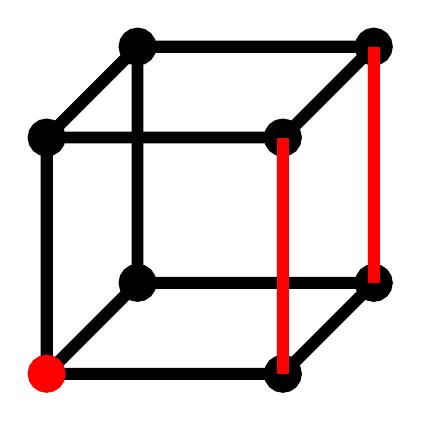
\begin{tikzpicture}[scale=3,line width=1.5mm]

                \draw [circle] (1,0,0) -- (1,0,1) -- (1,1,1) -- (1,1,0) -- cycle;
                \draw [circle] (0,0,0) -- (0,0,1) -- (0,1,1) -- (0,1,0) -- cycle;

                \draw [circle] (0,0,0)   -- (1,0,0)  -- (1,0,1)  -- (0,0,1)  -- cycle;
                \draw [circle] (0,1,0)   -- (1,1,0)  -- (1,1,1)  -- (0,1,1)  -- cycle;

                \draw [circle] (0,0,0)  node[draw, fill = black] (nodeA) {}  -- (1,0,0)  node[draw, fill = black] (nodeA) {}  -- (1,1,0)  node[draw, fill = black] (nodeA) {}  -- (0,1,0)  node[draw, fill = black] (nodeA) {}  -- cycle;
                \draw [circle] (0,0,1)  node[draw, fill = red, red] (nodeA) {}  -- (1,0,1)  node[draw, fill = black] (nodeA) {}  -- (1,1,1)  node[draw, fill = black] (nodeA) {}  -- (0,1,1)  node[draw, fill = black] (nodeA) {}  -- cycle;

                \draw [red] (1,1,1) -- (1,0,1);
                \draw [red] (1,1,0) -- (1,0,0);

            \end{tikzpicture}

            $\Rightarrow $ ДНФ $ = x \lor \overline{x} \: \overline{y} \: \overline{z} = x \lor \overline{y} \: \overline{z}$

        \end{example}

        \begin{remark}
            Данный метод позволяет наглядно перебрать все ДНФ и найти минимальный

            С помощью алгебраических преобразований мы не сможем понять, что ответ самый оптимальный
        \end{remark}

        \begin{example}
            Алгебраические преобразования

            $\overline{x} \: \overline{y} \: \overline{z} \lor x \: \overline{y} \: \overline{z} \lor xy \: \overline{z} = \overline{x} \: \overline{y} \: \overline{z} \lor x \: \overline{y} \: \overline{z} \lor x \: \overline{y} \: \overline{z} \lor xy \: \overline{z} = \overline{y} \: \overline{z} \lor x \: \overline{z}$

            Но тут непонятно, а вдруг можно сделать еще короче
        \end{example}

        \subsubsection{Двойственная функция}

        Пусть есть логическая функция: $f = B^n \rightarrow B = \{0, 1\}$

        Двойственная функция: $f^* = B^n \rightarrow B = \{0, 1\}$

        $f^*(x_1, x_2, \dots, x_n) = \overline{f(\overline{x_1}, \overline{x_2}, \dots, \overline{x_n})}$

        \begin{remark}
            Мир замены лжи на истину

            $$0 \leftrightarrow 1$$
        \end{remark}

        \begin{example}
            $f(x, y) = x \lor y$

            \begin{table}[h!]
                \centering
                \begin{tabular}{|c|c|c|}
                    \hline
                    $x$ & $y$ & $f$ \\ \hline
                    0      & 0   & 0   \\ \hline
                    0      & 1   & 1   \\ \hline
                    1      & 0   & 1   \\ \hline
                    1      & 1   & 1   \\ \hline
                \end{tabular}
            \end{table}

            Новый мир: $1 \rightarrow 0, 0 \rightarrow 1$

            \begin{table}[h!]
                \centering
                \begin{tabular}{|c|c|c|}
                    \hline
                    $x$ & $y$ & $f^*$ \\ \hline
                    1      & 1   & 1     \\ \hline
                    1      & 0   & 0     \\ \hline
                    0      & 1   & 0     \\ \hline
                    0      & 0   & 0     \\ \hline
                \end{tabular}
            \end{table}

            Получилось, что $(x \lor y)^* = xy$
        \end{example}

        \begin{example}
            $(x \lor y)^* = \overline{\overline{x} \lor \overline{y}} = \overline{\overline{x}} \: \overline{\overline{y}} = xy$
        \end{example}

        \begin{example}
            $(x + y)^* = \overline{\overline{x} + \overline{y}} = \overline{1 + x + 1 + y} = 1 + x + 1 + y + 1 = 1 + x + y = x \Leftrightarrow y$
        \end{example}

        \begin{remark}
            $f^{**}(x_1, x_2 \dots x_n) = \overline{f^*(\overline{x_1}, \overline{x_2} \dots \overline{x_n})} = \overline{\overline{f(x_1, x_2 \dots x_n)}} = f(x_1, x_2 \dots x_n)$
        \end{remark}

        \begin{corollary}
            $$(xy)^* = x \lor y$$

            $$(x \Leftrightarrow y)^* = x + y$$
        \end{corollary}

        \textbf{Теорема о композиции:}

        $f = f_0(f_1(x_1, \dots x_n), f_2(x_1, \dots x_n), \dots f_m(x_1, \dots x_n))$

        $f_i$ ~--- это функции от n переменных $(B^n \rightarrow B) (i = 1 \dots n)$

        $f_0 = B^m \rightarrow B$

        Тогда $f^*(x_1, \dots x_n) = f^{*}_{0}(f^{*}_{1}(x_1, \dots x_n), f^{*}_{2}(x_1, \dots x_n), \dots f^{*}_{m}(x_1, \dots x_n))$

        \textbf{Доказательство:}

        $f^* = \overline{f(\overline{x_1}, \dots \overline{x_n})} =  \overline{f_0(f_1(\overline{x_1}, \dots \overline{x_n}), f_2(\overline{x_1, \dots \overline{x_n}}) \dots f_m(\overline{x_1}, \dots \overline{x_n}))} = f_0^*(\overline{f_1(\overline{x_1, \dots \overline{x_n}}), \overline{f_2(\overline{x_1}, \dots \overline{x_n})}, \dots \overline{f_m(\overline{x_1}, \dots \overline{x_n})}}) $

        \begin{corollary}
            Если есть $f(x_1, \dots x_n)$ ~--- записано, как логическое выражение с $\cdot, \: \lor, \: \neg, \: +, \: \Leftrightarrow$, то $f^*$ ~--- также выражение, но связки заменяются на двойственные узлы

            $$\lor \leftrightarrow *$$

            $$+ \leftrightarrow \Leftrightarrow$$

            $$\neg \leftrightarrow \neg$$

            так как $(\overline{x})^* = \overline{x}$
        \end{corollary}

        \begin{example}

            $$f(x, y, z) = \overline{x \lor \overline{y} \: z} \Leftrightarrow (x + y + z)$$

            $$f^*(x, y, z) = (\overline{x \cdot (\overline{y} \: z)}) + (x \Leftrightarrow y \Leftrightarrow z)$$
        \end{example}

        \begin{example}

            $$f(x_1, \dots x_n) = 1$$

            $$\Rightarrow f^*(x_1, \dots x_n) = \overline{1} = 0$$

            $$1^* = 0; 0^* = 1$$
        \end{example}

        \subsubsection{Конъюнктивно-нормальная форма КНФ}

        \begin{definition}
            Конъюнктивно-нормальная форма ~--- еще одна нормальная форма, похожая на ДНФ
        \end{definition}

        \begin{definition}
            Литерал ~--- это как и раньше, переменные или отрицательные переменные

            $$x, y, \overline{x}, \: \overline{y}$$
        \end{definition}

        \begin{definition}
            Дизъюнкт ~--- дизъюнкция литералов

            $$x \lor y; \: x \lor y \lor \overline{z}; \: x \lor \overline{z}; \: \overline{x}$$

            $$\cancel{xy}, \cancel{x \lor yz}$$
        \end{definition}

        \begin{definition}
            КНФ ~--- это конъюнкция нескольких дизъюнктов

            $$(x \lor y)(y \lor \overline{z});$$

            $$(x \lor \overline{y} \lor z)(\overline{y} \lor \overline{z})(\overline{x})$$

            $$\cancel{xy \lor z}$$

            $$x \lor y \lor z$$ ~--- 1 дизъюнкт

            $$xyz$$ ~--- 3 дизъюнкта
        \end{definition}

    \end{sloppypar}

    \begin{definition}
        У любой логической функции есть КНФ, её можно построить по таблице истинности
    \end{definition}

    \textbf{Доказательство}

    Заметим,что если вычислить (КНФ$)^{*}$ (двойственную к КНФ), то получим ДНФ

    \begin{example}
        $[(x \vee y \vee z)(x \vee \bar{y})(\bar{y} \vee \bar{z})]^{*} = (xyz)\vee(x\bar{y})\vee(\bar{y}\bar{z})$

        И наоборот (ДНФ$)^{*} = $ КНФ
    \end{example}

    Итого, чтобы получить КНФ для функции f, надо построить двойственную функцию
    к ДНФ это функции. Отсюда следует, что КНФ всегда существует

    \begin{example}
        f(x,y,z) = xy $\Leftrightarrow$ z

        \begin{table}[h!]
            \centering
            \begin{tabular}{|c|c|c|c|c|c|}
                \hline
                $x$ & $y$ & $z$ & $xy$ & $f$ & $f^{*}$ \\ \hline
                0     & 0   & 0   & 0    & 1   & 0       \\ \hline
                0     & 0   & 1   & 0    & 0   & 1       \\ \hline
                0     & 1   & 0   & 0    & 1   & 1       \\ \hline
                0     & 1   & 1   & 0    & 0   & 0       \\ \hline
                1     & 0   & 0   & 0    & 1   & 1       \\ \hline
                1     & 0   & 1   & 0    & 0   & 0       \\ \hline
                1     & 1   & 0   & 1    & 0   & 1       \\ \hline
                1     & 1   & 1   & 1    & 1   & 0       \\ \hline
            \end{tabular}

        \end{table}


        Выпишем значения xyz из строчек, где $f^{*} = 1$

        $\bar{x}\bar{y}z$ \quad $x\bar{y}\bar{z}$ \quad $\bar{x}y\bar{z}$ \quad $xy\bar{z}$


    \end{example}

    Вспомним определение $f^{*}(x,y,z) = \overline{f(\bar{x},\bar{y},\bar{z})}$

    $f^{*}(0,0,0) = \overline{f(1,1,1)}$

    Итого: $f^{*}$ = $\bar{x}\bar{y}z \vee \bar{x}y\bar{z} \vee x\bar{y}\bar{z} \vee xy\bar{z}$

    $f^{*}(0,0,1) = \overline{f(1,1,0)}$

    $f^{*}(0,1,0) = \overline{f(1,0,1)}$

    По теореме о композиции

    $f = (\bar{x} \vee \bar{y} \vee z)(\bar{x} \vee y \vee \bar{z})(x \vee \bar{y} \vee \bar{z})(x \vee y \vee \bar{z})$

    Получение КНФ по таблице истинности без двойственной функции

    f(x,y,z) = xy $\Leftrightarrow$ z

    \begin{table}[h!]
        \centering
        \begin{tabular}{|c|c|c|c|}
            \hline
            $x$ & $y$ & $z$ & $f = xy \Leftrightarrow z $ \\ \hline
            0     & 0   & 0 & 1                           \\ \hline
            0     & 0   & 1 & 0                           \\ \hline
            0     & 1   & 0 & 1                           \\ \hline
            0     & 1   & 1 & 0                           \\ \hline
            1     & 0   & 0 & 1                           \\ \hline
            1     & 0   & 1 & 0                           \\ \hline
            1     & 1   & 0 & 0                           \\ \hline
            1     & 1   & 1 & 1                           \\ \hline
        \end{tabular}
    \end{table}


    При x y z = 1 1 0, f= xy $\Leftrightarrow$ z $\leftarrow$ $\bar{x}\lor\bar{y}\lor z$

    для 1 - отрицание, для 0 - нет отрицания

    Итого: Чтобы построить ДНФ:

    - строки с 1, $0 \leftrightarrow \bar{x}\bar{y}\bar{z}$

    \qquad \qquad \qquad $1 \leftrightarrow xyz$

    Чтобы получить КНФ:

    - строки с 0, 0 $\leftrightarrow xyz$

    \qquad \qquad \qquad 1 $\leftrightarrow \bar{x}\bar{y}\bar{z}$

    \begin{example}
        f = x+y

        \begin{table}[h!]
            \centering
            \begin{tabular}{|c|c|c|}
                \hline
                $x$ & $y$ & $x+y$ \\ \hline
                0     & 0   & 0     \\ \hline
                0     & 0   & 1     \\ \hline
                0     & 1   & 1     \\ \hline
                0     & 1   & 0     \\ \hline
            \end{tabular}
        \end{table}


        Нули в: $x \lor y \qquad \bar{x} \lor \bar{y}$

        $f = (x\lor y)(\bar{x} \lor \bar{y})$


    \end{example}

    \begin{remark}
        Для функции записанной в форме КНФ, можно поставить задачу "выполнимости".

        Вопрос: может ли значение быть = 1

        - не известно решений, принципиально эффективней полного перебора значений

    \end{remark}

    \begin{example}
        $(x \lor y \lor z)(x \lor \bar{y})(y \lor \bar{z})(\bar{x} \lor \bar{z}) = 1$

        x = 1

        y = 1 \qquad подходит

        z = 0

        Cледовательно эта формула выполнима при таком наборе


    \end{example}

    Многие задачи, головоломки сводятся к задаче выполнимости

    \begin{example}
        Прицнцип Дирихле

        Если есть n клеток и в них n+1 заяц, то $\exists$ клетка, где зайцев $\geqslant$ 2.

        при n = 2: i = 1 или 2 (клетка) \qquad $x_{ij} $ - в клетке i сидит заяц j

        \qquad \qquad \quad j = 1 или 2 или 3 заяц

        Попробуем записать, что в каждой клетке $\leqslant$ 1 зайца

        а) каждый заяц ровно в одной клетке

        $x_{11} \oplus x_{21}$ - заяц 1

        $x_{12} \oplus x_{22}$ - заяц 2

        $x_{13} \oplus x_{23}$ - заяц 3

        б) в каждой клетке не больше 1 зайца

        \begin{table}[h!]
            \centering
            \begin{tabular}{|c|c|c|c|}
                \hline
                кл/з & $1$      & $2$      & $3$      \\ \hline
                1      & $x_{11}$ & $x_{12}$ & $x_{13}$ \\ \hline
                2      & $x_{21}$ & $x_{22}$ & $x_{23}$ \\ \hline
            \end{tabular}
        \end{table}

        если есть 2 зайца, то один из конъюнктов: = 1

        $\overline{x_{11}x_{12} \lor x_{11}x_{13} \lor x_{12}x_{13}} \longleftarrow$ в кл $1 \leqslant 1$ зайца

        $\overline{x_{21}x_{22} \lor x_{21}x_{23} \lor x_{22}x_{23}} \longleftarrow$ в кл $2 \leqslant 1$ зайца

        Соединяем все утверждения:

        $(x_{11} + x_{21})(x_{12} + x_{22})(x_{13} + x_{23})(\overline{x_{11}x_{12} \lor x_{11}x_{13} \lor x_{12}x_{13}})(\overline{x_{21}x_{22} \lor x_{21}x_{23} \lor x_{22}x_{23}}) = 0$ всегда из принципа Дерихле

        $(x_{11} \lor x_{21})(\overline{x_{11}} \lor \overline{x_{21}})(x_{12} \lor x_{22})(\overline{x_{12}} \lor \overline{x_{22}})(x_{13} \lor x_{23})(\overline{x_{13}} \lor \overline{x_{23}})(\overline{x_{11}} \lor \overline{x_{12}})(\overline{x_{11}} \lor \overline{x_{13}})(x_{12} \lor x_{13})(\overline{x_{21}} \lor \overline{x_{22}})(\overline{x_{21}} \lor \overline{x_{23}})(\overline{x_{22}} \lor \overline{x_{23}})$

        $\longleftarrow$
        Берем программу, которая решает КНФ задачу выполнимости. Она скажет - невозможно.

    \end{example}

    \subsubsection{Класс замкнутости}

    Повторим: Логическая функция: f: $\beta^{n} \rightarrow \beta$

    $\beta = \{0,1\}$

    \begin{definition}
        Класс ~-- это множество логических функций.
    \end{definition}

    \begin{example}

        $K_{1} = $ класс функций: от двух переменных
        $K_{2} = $ класс функций такой, что $f(x,y) = f(y,x)$

        $f(x,y) = x \lor y \in K_{1}, \in K_{2}$

        $g(x,y) = x \Rightarrow y \in K_{1} \notin K_{2}$

        $K_{3}:$ класс функций $f(x,...) = f(\overline{x}, ...)$
        функции, которые не зависят от первой переменной

        $f(x,y,z) = y \Rightarrow z \in K_{3}$

        $f(x,y,z) = (x \Rightarrow y) \lor z \notin K_{3}$

        $f(x,y,z) = x\bar{x} \lor y \lor z \in K_{3}$ \quad $(x \bar{x})$

        $K_{4}: \{f(x,y) = x \lor y;$  $ g(x,y) = x \Rightarrow y\}$

    \end{example}

    \begin{definition}
        Замыкание класса

        $K = \{f_{1},f_{2},\dots\}$ ~--- класс функции

    \end{definition}
    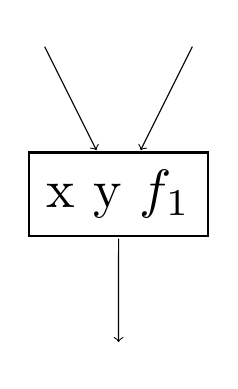
\begin{tikzpicture}
        \node (first_diag)[scale = 1.5, style = {thick, draw = black}]
        [scale = 1.3] at ( 0,0) {x y $f_{1}$};
        \node (1) at ( 1,2) {};
        \node (2) at ( -1,2) {};
        \node (3) at ( 0,-2) {};
        \path(1) edge[->] (first_diag);
        \path(2) edge[->] (first_diag);
        \path(first_diag) edge[->] (3);
    \end{tikzpicture}
    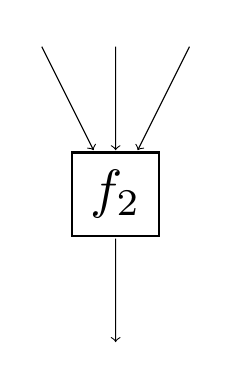
\begin{tikzpicture}
        \node (first_diag)[scale = 1.5, style = {thick, draw = black}]
        [scale = 1.3] at ( 1,1) {$f_{2}$};
        \node (1) at ( 0,3) {};
        \node (2) at ( 2,3) {};
        \node (3) at ( 1,3) {};
        \node (4) at ( 1,-1) {};
        \path(1) edge[->] (first_diag);
        \path(2) edge[->] (first_diag);
        \path(3) edge[->] (first_diag);
        \path(first_diag) edge[->] (4);
    \end{tikzpicture}

    $K^{*}$ ~--- замыкание класса - это класс состоящий из всех композиций функций из K


    \frame{$f_{1}(f_{2})(f_{1}(x,y),y,z),z)$} ~--- композиция

    если есть функции, подставляем друг в друга, получаем композицию

    \begin{example}
        $:1) K = \{0,\bar{x}\}$ \quad (0 - f() $\bar{x} - g(x)$)

        $K^{*} = \{ f(), g(f()), g(g(f())), g(g(g(f())))\}$
    \end{example}
    \begin{example}
        $K = \{\bar{x}\}$ возьмем класс только из отрицательных

        $K^{*} = \{ \bar{x}, x\}$

        $K = \{ g(x), g((g(x))), g(g(g(x \dots 1, \dots )))\}$
    \end{example}
    \begin{example}
        $K^{*}=\{ \bar{x}$,$ x \lor y$,$ xy \}$  $\quad K^{*} = \{ $,$ \dots$,$ \forall$, функция $\}$
    \end{example}

    \begin{definition}

        Если К - класс:

        $K^{*} = \alpha$, то \frame{К - полный}, где $\alpha$ ~--- все логические функции

        Вывод: $K = \{ \bar{x}, x \lor y, xy\}$ ~--- полный

    \end{definition}
    \begin{example}

        $K = \{\bar{x}, x \lor y \}$, где $f(x) = \bar{x}$, $g(x, y) = x \lor y$
    \end{example}

    $xy = \overline{\overline{xy}} = \overline{\overline{x} \lor \overline{y}}
    = f(g(f(x),f(y)))$  % need check

    Значит $K^{*}$ ~--- тоже полный


    \begin{definition}
        Замкнутый класс ~~- K замкнут, если $K^{*} = K$
    \end{definition}

    Свойства замыкания:

    1. $K_{1} \subset K_{2}$, тогда $K_{1}^{*} \subset K_{2}^{*}$

    \textbf{Доказательство:}

    Если есть f $\in K_{1}^{*} \Rightarrow f = $ композиция $f_{1} \in K_{1} \Rightarrow$
    f - композиция $(f_{i} \in K_{2}) \Rightarrow f \in K_{2}^{*} $ чтд.

    2.Если $K_{1} \subset K_{2}$ и $K_{1}$ - полный, то $K_{2}$ - полный

    \textbf{Доказательство:}

    $K_{1} \subset K_{2} \Rightarrow K_{1}^{*} \subset K_{2}^{*} \Rightarrow \alpha
    \subset K_{2}^{*} \Rightarrow K_{2}^{*} = \alpha
    $

    3. Пусть $K_{1}$, $K_{2}$ ~~- замкнутое, тогда $K_{1} \cap K_{2}$ ~~- тоже замкнутые

    \textbf{Доказательство:}

    Пусть есть $f = (K_{1} \cap K_{2})^{*} $ ~~- композиция

    $f_i \in (K_{1} \cap K_{2})$

    а) $\Rightarrow f_i $ ~~- композиция $ f_i = K_1 \Rightarrow f \in K_{1}^{*}$

    б) $\Rightarrow f_i $ - композиция $f_i = K_2 \Rightarrow f \in K_{2}^{*}$

    Из а и б следует, что $ f \in K_{1}^{*} \cap K_{2}^{*} = K_{1} \cap K_{2}$

    Итог: $f \in (K_{1} \cap K_{2})^{*} \Rightarrow f \in K_{1} \cap K_{2}$

    $\Rightarrow    (K_{1} \cap K_{2})^{*} \subset K_{1} \cap K_{2}$,
    по $K_{1} \cap K_{2} \subset (K_{1}
    \cap K_{2})^{*}$

    $\Rightarrow K_{1} \cap K_{2} = (K_{1} \cap K_{2})^{*}$

    $\Rightarrow K_{1} \cap K_{2} $ - замкнут

    \begin{remark}
        $K_{1}$ и $K_{2}$ - замкнутые $\Rightarrow K_{1} \cup K_{2} $ - замкнутый
    \end{remark}

    4. $K^{*} = K^{**}$ для любого класса функций

    \subsubsection{Примеры замкнутых классов}

    1. $T_{0}$ - класс функций, "сохраняющих ноль" $f \in T_{0} \Leftrightarrow$  если
    $f(0,....0) = 0$

    $x*y \in T_{0}$

    $x+y \in T_{0}$

    $\bar{x} \notin T_{0}$

    $x \Rightarrow y \notin T_{0}$

    $xy + xz + yz \in T_{0}$

    \textbf{Утверждение:} $T_{0} $ - замкнут

    \textbf{Доказательство:}

    $\sqsupset f \in T_{0}^{*}$, проверим, что $f \in T_{0}$

    $\Rightarrow T_{0}^{*} \subset T_{0}$

    $\Rightarrow T_{0}^{*} = T$

    f - комп $f_{i}$, $f_{i} \in T_{0}$

    $f_{1}(f_{2}(...)f_{3}(f_{4}(...)),...)$ - композиция

    подставим все 0

    $\Rightarrow f(0,....0) = 0 \Rightarrow f \in T_{0} $ чтд

    \begin{example}
        $f_{1}(x,y) = x*y$ \qquad $f_{1} \in T_{0} f_{2} \in T_{0}$

        $f_{2}(x,y) = x+y$ \qquad $f_{1}(f_{2}(f_{1}(x,f_{2}(y,y)),y)f_{1}(z,z))$

        $x(y+y)$

        $f(x,y,z) = (x(y+y)+y)*z*z$

        $f(0,0,0) = 0$

        2. Класс $T_{1}$ - сохраняющие 1

        $f \in T_{1}$, если $f(1,...1) = 1$

        $x*y \in T_{1}$

        $x+y \notin T_{1}$

        $x+y+z \in T_{1}$

        $\bar{x} \notin T_{1}$

        $x \Rightarrow y \in T_{1}$

        $xy + xz + yz \in T_{1}$

        \begin{proposition}
            $T_{1}$ - замкнут
        \end {proposition}


        \textbf{Доказательство:} смотри $T_{0}$

        3. Класс $\frame{\&}$

        $f \in \frame{\&}$, если f можно записать как конъюнкцию нескольких переменных

        $f(x,y,z) = yz$

        $g(x,y,z) = xyz$

        $h(x,y,z) = xz$

        $i(x,y,z) = z$

        0

        1

        Все это $\in \frame{\&}$

        \begin{proposition}
            Класс $\frame{\&}$ замкнут
        \end{proposition}

        Композиция $f_{i} \in \frame{\&}$

        $f_1(...,\frame{...},...,\frame{...}) = $ арг2 * арг4 = подаргумент1* подаргумент2* ... * подаргумент =
        пер * пер * пер * пер... (произвольная переременная)

        пер может быть 0 или 1

        \begin{proposition}
            $\frame{\&} = \{\&,0,1\}^{*}$

            по определению замыкания

            $\{f_{1}(x,y) = x*y$

            $f_{2}() = 0$

            $f_{3}() = 1\}$

        \end{proposition}

        4. \frame{V} - дизъюнкция переменных и 0, 1

        \frame{V} = $\{V,0,1\}^{*}$

        \begin{proposition}

            $\frame{V} $ - замкнут

        \end{proposition}

        \textbf{Доказательство 1: }

        смотри доказательство $\frame{\&}$


        \textbf{Доказательство 2: }

        $\frame{V} = \{V,0,1\}^{*}$
        $\Rightarrow \frame{V}^{*} = \{V,0,1\}^{**} = \{V,0,1\}^{*} = \frame{V}$ свойства замыкания

    \end{example}

    \textbf{Доказательство: } $\sqsupset  f \in K^{*} \Rightarrow f - $ комп $f_{i}
    \Rightarrow f_{i} \in K^{*}
    $

    $ f = f_{1} (f_2(...)...) = g_{1}(g_{2}(h_{1}...)) \in k^{*}
    $

    \qquad $\uparrow$ \quad $\uparrow$ \qquad комп $g_{1} \in K^{*}$

    $g_{i} \in K $ $h_{i} \in K$

    $\Rightarrow f \in K^{*} \Rightarrow K^{*} = K^{**}$

    Следствие: $\forall K$ - класс $K^{*}$ - замкнут

    если класс замкнут он станет замкнутым

    5. Класс u (unit) : 0,1,$f(x,...x_{n}) = x_{i}$ или  $\overline{x_{i}}$

    $f(x,y,z) = \bar{z}$

    $f(x,y,z,t) = x$

    $f(x) = x f(x) = \bar{x}$

    Все это $\in u$

    6. Класс $1^{\infty}$ $f(x_{1}...x_{n}) \leqslant x_{i} $

    \qquad $0^{\infty} f(x...x_{n}) \geqslant x_{i}$

    $x*y \leqslant x$ \qquad $xy \in 1^{\infty}$

    \quad $\leqslant y$

    $x \lor y \geqslant x$ \qquad $x \lor y \in 0^{\infty}$

    \quad $\geqslant y$

    $x \Rightarrow y \geqslant y$ \quad $x \Rightarrow y \in 0^{\infty} $

    $x \Rightarrow y \leqslant y $

    \qquad $x=0$

    \qquad $y=0$

    $x \Rightarrow y \notin 1^{\infty}$

    7. L - линейная функция L = $\{0,1,+\}^{*}$

    Все функции из констант и сложения

    $x+y \in L$

    $x+y + z \in L$

    $1+x \in L$

    $\bar{x} \in$

    $x * y \in L$

    (L - линейные многочлены Жегалкина, степени $\leqslant$ 1)

    \textbf{Доказательство: } $ x * y$ имеет многочлены Жегалкина $x*y$

    он единственный $\Rightarrow $ не существует линейного многочлена Жегалкина %do

    8. S - самодвойствейнные функции

    $f \in S$, если f = $f^{*}$ \quad ($f^{*} $ - двойственные)

    Если функция равна своей двойственной, то она самодвойтсвенная

    \begin{example}
        $x*y \notin S$

        $x \lor y \notin S$

        $x \in S$

        $\bar{x} \in S$

        $x \Rightarrow y \notin S $ т.к. $(x \Rightarrow y)^{*} = (\bar{x} \lor y)^{*} = \bar{x}*y \neq \bar{x} \lor y$

        $x = 1$
    \end{example}
    Функция честного голосования $y = 1$ от 3 ёх переменных. $0 \neq 1$

    $vote(x,y,z) = 1$,  если 1 - иц больше $x + y + z \geq z$

    \qquad \quad \quad \quad \quad \quad 0, если 0 - ей больше $x + y + z \leq 1$

    $vote(x,y,z)$ : Таблица истинности


    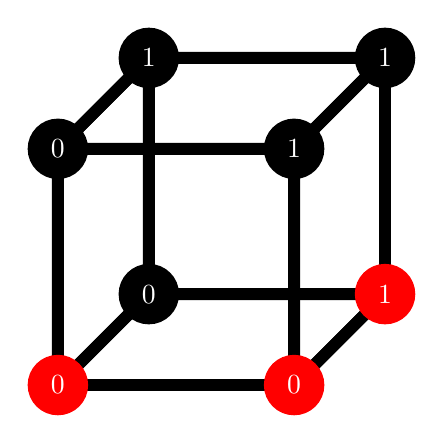
\begin{tikzpicture}[scale=3,line width=1.5mm]

        \draw [circle] (1,0,0) -- (1,0,1) -- (1,1,1) -- (1,1,0) -- cycle;
        \draw [circle] (0,0,0) -- (0,0,1) -- (0,1,1) -- (0,1,0) -- cycle;

        \draw [circle] (0,0,0)   -- (1,0,0)  -- (1,0,1)  -- (0,0,1)  -- cycle;
        \draw [circle] (0,1,0)   -- (1,1,0)  -- (1,1,1)  -- (0,1,1)  -- cycle;

        \draw [circle] (0,0,0)  node[draw, fill = black] (nodeA) {\textcolor{white}{0}}  -- (1,0,0)  node[draw, fill = red, red] (nodeA) {\textcolor{white}{1}}  -- (1,1,0)  node[draw, fill = black] (nodeA) {\textcolor{white}{1}}  -- (0,1,0)  node[draw, fill = black] (nodeA) {\textcolor{white}{1}}  -- cycle;
        \draw [circle] (0,0,1)  node[draw, fill = red, red] (nodeA) {\textcolor{white}{0}}  -- (1,0,1)  node[draw, fill = red, red] (nodeA) {\textcolor{white}{0}}  -- (1,1,1)  node[draw, fill = black] (nodeA) {\textcolor{white}{1}}  -- (0,1,1)  node[draw, fill = black] (nodeA) {\textcolor{white}{0}}  -- cycle;

    \end{tikzpicture}

    $vote(x,y,z) \in S$?

    $(xy \lor xz \lor yz)^{*} = (x \lor y)(x \lor z)(y \lor z) =? xy \lor xz \lor yz$

    Раскроем скобки:

    $xxy \lor xxz \lor xzy \lor xzz \lor yxy \lor yxz \lor yzy \lor yzz =
    xy \lor xz \lor xyz \lor xz \lor xy \lor xyz \lor yz \lor yz = xy \lor
    xz \lor yz \lor xyz = xy \lor xz \lor yz(1 \lor x) = xy \lor xz \lor yz$

    т.е. vote = $vote^{*}$

    или проверим таблицой истинности:

    читаем снизу вверх, заменяя 0 на 1

    \begin{table}[h!]
        \begin{tabular}{|c|c|c|}
            \hline
            $xyz$ & $vote$ & $vote^{*}$ \\ \hline
            000     & 0      & 0          \\ \hline
            001     & 0      & 0          \\ \hline
            010     & 0      & 0          \\ \hline
            011     & 1      & 1          \\ \hline
            100     & 0      & 0          \\ \hline
            101     & 1      & 1          \\ \hline
            110     & 1      & 1          \\ \hline
            111     & 1      & 1          \\ \hline
        \end{tabular}
    \end{table}

    \begin{proposition}

        S - замкнут

        $\sqsupset f \in S^{*} f = $композиция $f_{i} \in S$

        $f = f_{i}(f_{2}(...),f_{3}(...),f_{4}(...))$

    \end{proposition}

    \begin{definition}

        Высота композиции

        $f(x,y,z)$ - высота 1 (1 ф-ия)

        $f(g(x,y),y,z)$ - высота 2

        $g(x,y) - 1$

        $f(g(x,y),y,z) - 2$
    \end{definition}


    \begin{example}
        $f(g(h(x),y),h((h(x)),y))$

        $g(h(x),y)$ - 2

        $h(h(x))$ - 2

        $f(g(h(x),y),h((h(x)),y))$ - 3

    \end{example}

    $f^{*} = f_{1}^{*}(f_{2}^{*}(...),  ,f_{n}^{*}(...))$ - теория о композиции

    но $f_{i} \in S \Rightarrow f_{i}^{*} = f_{i}$

    $= f_{i}(f_{2}(...),...f_{n}(...)) = f$

    т.е $f^{*} = f \Rightarrow f \in S$

    9. Монотонные функции

    $f(x_1, \dots, x_n) \in M$, если $\forall i \quad x_i \geq y_i$

    $\Rightarrow f(x_1, \dots, x_n) \geq f(y_1, \dots, y_n)$

    \textbf{Примеры:}
    \begin{enumerate}
        \item{
            $f_1(x) = \overline{x} \qquad f_1 \notin M$, так как $f_1(1) = 0, f(0) = 1$.
            $1$ в аргументе функции $\geq 0$, но $0 < 1$ в значение функции

        }
        \item{
            $f_2(x, y) = x \Rightarrow y \qquad f_2 \notin M$, так как $f_2(1,0) = 0, f(0,0) = 1$.
            $1,0$ в аргументе функции $\geq 0,0$, но $0 < 1$ в значение функции
        }
        \item{
            $f_3(x, y) = x + y \qquad f_3 \notin M$, так как $f_3(1,1) = 0, f(1,0) = 1$.
            $1,1$ в аргументе функции $\geq 1,0$, но $0 < 1$ в значение функции
        }
        \item $f_4(x, y) \in M$
        \item $f_5(x, y) \in M$
        \item $f_6(x, y, z) = xy \lor xz \lor yz \quad \in M$ ~--- функция голосования
    \end{enumerate}

    \textbf{Наглядный способ проверки монотонности}

    Функция монотонна, когда все стрелки:
    \begin{enumerate}
        \item из 0 в 0
        \item из 0 в 1
        \item из 1 в 1
    \end{enumerate}

    \begin{example}
        $x * y$

        Данная функция монотонна

        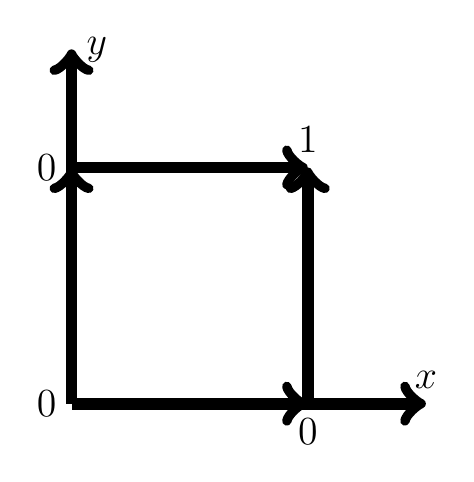
\begin{tikzpicture}
            [scale=3,line width=1.5mm, ->]
            \draw (0, 0) node [left] {\Large $0$} -- (0, 1.5) node [right] {\Large $y$};
            \draw (0, 0) -- (0, 1) node [left] {\Large $0$};
            \draw (0, 0) -- (1, 0) node [below] {\Large $0$};
            \draw (0, 0) -- (1.5, 0) node [above] {\Large $x$};
            \draw (0, 1) -- (1, 1) node [above] {\Large $1$};
            \draw (1, 0) -- (1, 1);
        \end{tikzpicture}
    \end{example}

    \begin{example}
        $x \lor y$

        Данная функция тоже монотонна

        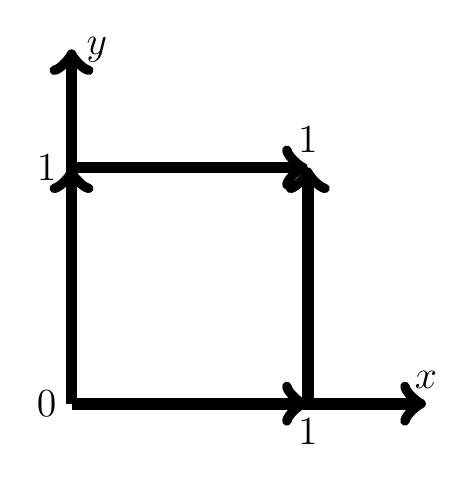
\begin{tikzpicture}
            [scale=3,line width=1.5mm, ->]
            \draw (0, 0) node [left] {\Large $0$} -- (0, 1.5) node [right] {\Large $y$};
            \draw (0, 0) -- (0, 1) node [left] {\Large $1$};
            \draw (0, 0) -- (1, 0) node [below] {\Large $1$};
            \draw (0, 0) -- (1.5, 0) node [above] {\Large $x$};
            \draw (0, 1) -- (1, 1) node [above] {\Large $1$};
            \draw (1, 0) -- (1, 1);
        \end{tikzpicture}
    \end{example}

    \begin{proposition}
        $M$ ~-- замкнут

        То есть если $f_i$ ~-- мотонна, то $f(x_1, \dots x_n) = f_1(f_2(\dots) \dots f_m(\dots))$

        $f(y_1, \dots y_n) = f_1(f_2(\dots) \dots f_m(\dots))$

        $x_1 \dots x_n \geq y_1 \dots y_n$

        То где-то в глубине $x_i$ будут $\geq y_i \Rightarrow$ внутри будут получаться значения функции $f_i(x \dots) \geq f_i(y \dots)$
    \end{proposition}

    \begin{remark}
        Классы из примеров выше все неполные
    \end{remark}

    \begin{example}
        $L = L^* \quad x \cdot y$

        Всегда были примеры функций не из классов

        $xy \notin L$

        $xy \notin S$

        $\overline{x} \notin T_0$

        $\overline{x} \notin T_1$

        $\overline{x} \notin M$
    \end{example}

    \subsubsection{Теорема Поста}

    \begin{theorem}
        \textbf{Поста}

        (Позволяет понять, полный класс или нет)

        $K$ ~-- полный тогда и только тогда, когда

        $\exists f_1 \in K: \quad f_1 \notin T_0$

        $\exists f_2 \in K: \quad f_2 \notin T_1$

        $\exists f_3 \in K: \quad f_3 \notin L$

        $\exists f_4 \in K: \quad f_4 \notin M$

        $\exists f_5 \in K: \quad f_5 \notin S$
    \end{theorem}

    \begin{example}
        $K = \{ \overline{x}; x + y \}$

        $\overline{x} \notin T_0, T_1$

        но $\overline{x} \in L$ и $x + y \in L \Rightarrow$

        $K$ ~-- не полный
    \end{example}

    \begin{example}
        $K = \{ \overline{x}; x \lor y \}$

        $\overline{x} \notin T_0, T_1, M$

        $\overline{x} \in S, L \quad $ но $x \lor y \notin L, S \Rightarrow$

        $K$ ~-- полный по теореме Поста
    \end{example}

    \textbf{Доказательство в одну сторону:}

    $\Rightarrow$ если $K$ полный, от противного

    Пусть все $f \in K$ отличие, что
    $f \in T_0$

    $ \Rightarrow K \subset T_0$

    $\Rightarrow K^* \subset T^*_0$

    $\Rightarrow K^* \subset T_0 \nleq \alpha$, где $\alpha$ ~-- все функции

    $\Rightarrow \leq \alpha$

    \textbf{Доказательство в другую сторону:}

    Будем выражать через $f_1; f_2; f_3; f_4; f_5$ все другие возможные

    Достаточно будет выразить только $\{ \overline{x}, x \cdot y\}$ (тогда есть $x \lor y = \overline{\overline{x} \cdot \overline{y}}$)

    $\Rightarrow$ есть все ДНФ.

    \textbf{Шаг 1:}
    Давайте выразим 0, 1, $\overline{x}$

    Берем $f_1(x_1 \dots x_n) = $
    $\left[
    \begin{gathered}
        1, x = 0 (f_1 \notin T_0) \hfill
        \\
        0 \: or \: 1; x = 1 \hfill
        \\
    \end{gathered}
    \right.$
    $ = 0$ или $\overline{x}$

    $f_2(x_1, x_2 \dots x_n) \notin T_1 = $
    $\left[
    \begin{gathered}
        0 \: or \: 1, x = 0 \hfill
        \\
        0; x = 1 \hfill
        \\
    \end{gathered}
    \right.$
    $ = \overline{x}$ или $0$

    \textbf{Пояснение:}

    $f(x, y, z) = x \Rightarrow yz \quad f(x, x, x) = 1$

    $f(0, 0, 0) = 1, f \notin T_0$

    $f(x, x, x) = 1$

    $0 = f_2(x_1 \dots x_n), \: 1 =    f_1(x_1, \dots x_n)$

    $0 = f_2(x_1, \dots x_n), \: \overline{x} = f_1(x_1, \dots x_n), \: 1 = \overline{0} = f_1(f_2(x_1, \dots x_n), f_2(x_1, \dots x_n), \dots) $

    $1 = f_2(x_1, \dots x_n), \: \overline{x} = f_1(x_1, \dots x_n), \: f_2(f_1(x_1, \dots x_n), f_1(x_1, \dots x_n), \dots)$

    $\overline{x} = f_2(x_1, \dots x_n), \: \overline{x} = f_1(x_1, \dots x_n)$

    Берем $f_4 \notin M$, где нарушена монотонность, для примера:

    $f_4(x_1 = y_1, x_2 = y_2, \dots, x_n > y_n) = 0_x \neq 1_y$

    $f_4(x_1, x_2, \dots x_n)$ переменная $X$, где $>$

    $f_4(x, y, z, t) = xy + zt \notin M$

    $f_4(1, 1, 1, 1) = 0 \quad f_4(1, 0, 1, 1) = 1$

    $1, 1, 1, 1 \geq 1, 0, 1, 1$

    $\Rightarrow f_4(1, x, 1, 1) = $
    $\left[
    \begin{gathered}
        1, x = 0 \hfill
        \\
        0; x = 1 \hfill
        \\
    \end{gathered}
    \right.$
    $ = \overline{x}$


    выражены $f_1(x_1, x_2 \dots x_n) = \overline{x} \quad f_2(x_1, x_2, \dots x_n) = \overline{x}$

    $f_5 \notin S$

    получим с ней 1 и 0

    Найдем нарушение $S$

    $f^*(x_1 \dots x_n) \neq f(x_1 \dots x_n)$

    $\overline{f(\overline{x_1}, \dots \overline{x_n})} \neq f(x_1, \dots x_n)$

    $f(\overline{x_1}, \overline{x_2}, \dots \overline{x_n}) = f(x_1, \dots x_n)$

    Рассмотрим $f_5(x; \overline{x}; x; \dots \overline{x}) = $

    (если $x_i = 0 \Rightarrow x \quad x_i = 1 \Rightarrow \overline{x}$)

    $= $
    $\left[
    \begin{gathered}
        f(x_1, x_2 \dots x_n) \: when \: x = 0 \hfill
        \\
        f(\overline{x_1}, \dots \overline{x_n}) \: when \: x = 1 \hfill
        \\
    \end{gathered}
    \right.$
    $ = 0$ или $1$

    \begin{example}
        $f(x, y, z) = x \lor yz \notin S$

        нужно найти $f(1, 0, 0) = f(0, 1, 1)$ (нарушение $S$)

        Рассмотрим $f(\overline{x}, x, x) = $
        $\left[
        \begin{gathered}
            f(1, 0, 0) = 1 \quad x = 0 \hfill
            \\
            f(0, 1, 1) = 1 \quad x = 1 \hfill
            \\
        \end{gathered}
        \right.$
        $ = 1$

        $f(\overline{x}, x, x) = \overline{x} \lor xx = \overline{x} \lor x = 1$

        если получили 0, то $\overline{0} = 1$ и наоборот
    \end{example}

    \textbf{Шаг 2:}

    Имеем $0, 1, \overline{x}$

    Надо $x \cdot y$ выразить

    Берем $f_3 \in L$

    $f_3(x_1, \dots x_n) = \dots + \dots + \dots + x_iy_j + \dots$

    Подставим $0; 1; x_i; x_j$

    Возьмем самое короткое слагаемое с $x_i \quad x_j$

    Для определенности $\exists$ это $x_1 \cdot x_2$

    $f_3(x_1 \dots x_n) = 1 + x_1 + x_2 + x_1x_2x_3\dots x_k + \dots$

    подставим $x_3 \dots x_k = 1$

    остальные $x_{k+1 \dots} = 0$

    $f(x_1, x_2, 1, 1, 1, 0, 0, 0, \dots 0) = C_1 + x_1x_2 + C_2x_1 + C_3x_2 + 0 \cdot x_1x_2 = $

    $g(x_1, x_2) = $
    $\left[
    \begin{gathered}
        x_1 x_2 \hfill
        \\
        1 + x_1 x_2 \hfill
        \\
        1 + x_1 + x_1 x_2 \hfill
        \\
        1 + x_2 + x_1 x_2 \hfill
        \\
        x_1 + x_1 x_2 \hfill
        \\
        x_2 + x_1 x_2 \hfill
        \\
        x_1 + x_2 + x_1 x_2 \hfill
        \\
    \end{gathered}
    \right.$


    если $g(x_1, x_2) = 1 + x_1 x_2$

    $\overline{g(x_1, x_2)} = x_1 x_2$ ~-- отрицание уже есть

    если $g(x_1, x_2) = 1 + x_1 + x_1 x_2 = 1 + x_2(1 + x_2)$

    тогда $\overline{g(x_1, \overline{x_2})} = 1 + (1 + x_1(1 + 1 + x_2)) = x_1 x_2$

    все случаи: $g(x_1, x_2) = C_1 + (x_1 + C_2) \cdot (x_2 + C_3)$

    \begin{example}
        $f_3(x, y, z) = x + yz$

        $f_3(0, x, y) = 0 + xy = xy$
    \end{example}

    \begin{example}
        $f_3(x, y, z) = x \Rightarrow yz = 1 + x + xyz$

        $f_3(x, y, 1) = 1 + x + xy = 1 + x(1 + y)$

        $\overline{f_3(x, \overline{y}, 1)} = xy$

        можно было

        $f_3(1, x, y) = 1 + 1 + xy = xy$
    \end{example}

    \begin{example}
        $f(x, y, z) = x \Rightarrow yz$


        $g(x, y) = x + y$

        $\notin T_0, T_1, L, M, S$

        Выражаем

        $f(x, x, x) = x \Rightarrow xx = 1$

        $g(x, x) = x + x = 0$

        Случай 0, 1, надо $\overline{x}$

        Выражаем $\overline{x}$

        $g(x, y) \notin M$

        $g(1, 0) = 1$

        $g(1, 1) = 0$

        $\Rightarrow g(1, x) = \overline{x}$

        $\Rightarrow \overline{x} = g(f(x, x, x), x)$

        Выражаем $x \cdot y$

        $f(x, y, z) = xx \Rightarrow yz = 1 + x + xyz$

        Догадаемся, что $f(1, x, y) = x \cdot y$

        Ответы: $\overline{x} = g(f(x, x, x), x) \quad x \cdot y = f(1, x, y)$
    \end{example}


    Полные наборы из одной функции (от двух переменных)

    $\{f(x,y)\}$ ~~~- полный

    По теореме Поста: $f(x,y) \notin $ L,M,S,$T_{0}$,$T_{1}$

    Таблица истинности для f:

    \begin{table}[h!]
        \begin{tabular}{|c|c|c|c|c|}
            \hline
            $xy$ & $f1$ & $f2$ & $f3$ & $f4$ \\ \hline
            00     & 1    & 1    & 1    & 1    \\ \hline
            01     & 0    & 0    & 1    & 1    \\ \hline
            10     & 0    & 1    & 0    & 1    \\ \hline
            11     & 0    & 0    & 0    & 0    \\ \hline
        \end{tabular}
    \end{table}

    1 строчка :

    xy $f_{1} f_{2} f_{3} f_{4}$

    00 1 1 1 1 $\notin T_{0}$

    4 строчка :

    xy $f_{1} f_{2} f_{3} f_{4}$

    11 0 0 0 0 $\notin T_{1}$


    $f_{2}(x,y) = \bar{y} \in L$

    $f_{3}(x,y) = \bar{x} \in L$

    $\Rightarrow f_{2},f_{3}$ не подходят

    $f_{1} = \overline{x \lor y}$ $ f_{4} = \overline{x * y}$

    $f_{1}^{*} = f_{4}$ \quad $f_{1},f_{4} \notin S$

    $f_{1} = \overline{x + y + xy} = 1 + x + y +xy \notin L$

    $f_{4} = 1+xy \notin L$

    $f_{1,4}(0,0) = 1 \notin M$

    $f_{1,4}(1,1) = 0 \notin M$

    Ответ: $\{\overline{x \lor y}\}$ ~~~- полный набор

    $\{x \downarrow y \}$ ~~~- стрелка пирса

    $\{x | y\}$ штриф шеффера

    x|x = $\bar{x}$

    $x|y = \overline{x*y} \Rightarrow \overline{x | y} = x * y \Rightarrow (x | y)|(x|y) = x*y $

    $x/y = \overline{xy} = \bar{x} \lor \bar{y} \Rightarrow \bar{x}/\bar{y} = x \lor y $

    $\Rightarrow (x/x)/(y/y) = x \lor y$

    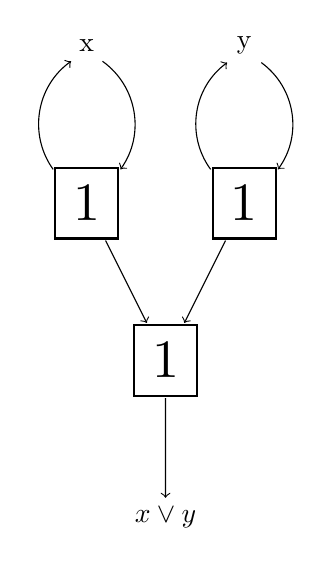
\begin{tikzpicture}
        \node (3_diag) at ( 1,4) {y};
        \node (4_diag) at (-1,4) {x};

        \node (1_diag)[scale = 1.5, style = {thick, draw = black}]
        [scale = 1.3] at ( 1,2) {1};

        \node (2_diag)[scale = 1.5, style = {thick, draw = black}]
        [scale = 1.3] at ( -1,2) {1};
        \node (first_diag)[scale = 1.5, style = {thick, draw = black}]
        [scale = 1.3] at ( 0,0) {1};
        \path(4_diag) edge[->,bend left=45] (2_diag);
        \path(2_diag) edge[->,bend left=45] (4_diag);
        \path(3_diag) edge[->,bend left=45] (1_diag);
        \path(1_diag) edge[->,bend left=45] (3_diag);
        \node (2) at ( -1,2) {};
        \node (3) at ( 0,-2) {$x \lor y$};
        \path(1_diag) edge[->] (first_diag);
        \path(2_diag) edge[->] (first_diag);
        \path(first_diag) edge[->] (3);
    \end{tikzpicture}


    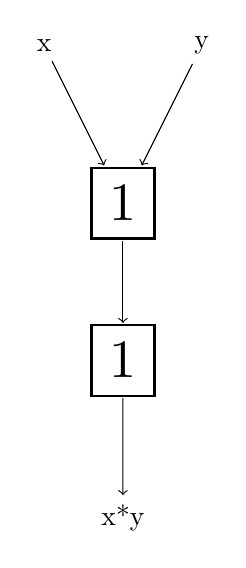
\begin{tikzpicture}

        \node (1_diag) at ( 1,2) {y};

        \node (2_diag) at ( -1,2) {x};
        \node (first_diag)[scale = 1.5, style = {thick, draw = black}]
        [scale = 1.3] at ( 0,0) {1};
        \node (2) at ( -1,2) {};
        \node (3)[scale = 1.5, style = {thick, draw = black}]
        [scale = 1.3] at ( 0,-2) {1};
        \node (4) at ( 0,-4) {x*y};
        \path(1_diag) edge[->] (first_diag);
        \path(2_diag) edge[->] (first_diag);
        \path(first_diag) edge[->] (3);
        \path (3) edge[->] (4);
    \end{tikzpicture}

    \subsubsection{Автоматическое доказательство теорем}

    Задача выполнимости: дана функция в КНФ

    $(x_{1} \lor x_{2} \lor \bar{x_{3}})(\bar{x_{1}} \lor \bar{x_{2}} \lor x_{3})(x_{1} \lor x_{4})$

    Эффективных алгоритмов для этой задачи нет

    ...

    -всегда 0

    -бывает 1

    \subsubsection{Логическое следствие}

    \begin{definition}
        $P_{1}(x_{1}...x_{k})...P_{n}(x_{1}...x_{k})$

        $n+1$ лог. функций (утверждений)

        Q($x_{1} ... x_{k}$)

        Q ~~~- логическое следствие $P_{1} ... P_{n}$, если для всех наборов значений $x_{i}$, когда все $P_{j}(x_{i}...x_{k}) = 1$

        $Q(x_{1}...x_{k})$ тоже 1

    \end{definition}


    \begin{example}
        $P_{1}(x,y,z)^{k=3} (x+y)\Leftrightarrow 0 $

        $P_{2}(x,y,z) = (y+z) \Leftrightarrow 1$

        $Q(x,y,z) = (x+z) \Leftrightarrow 1 $

        $0+1 = x+y+y+z=x+zy+z=1$


    \end{example}

    \begin{table}[h!]
        \begin{tabular}{|c|c|c|c|}
            \hline
            $xyz$ & $P_{1}$ & $P_{2}$ & $Q$ \\ \hline
            000     & 1       & 0       & 0   \\ \hline
            001     & 1       & 1       & 1   \\ \hline
            010     & 0       & 1       & 0   \\ \hline
            011     & 0       & 0       & 1   \\ \hline
            100     & 0       & 0       & 1   \\ \hline
            101     & 0       & 1       & 0   \\ \hline
            110     & 1       & 1       & 1   \\ \hline
            111     & 1       & 0       & 0   \\ \hline
        \end{tabular}
    \end{table}

    Есть 2 набор (001) и (110), где $P_{2}$ ~~~- истина

    Q должно быть тоже истина.

    \begin{remark}
        Q - логическое сложение $P_{1},P_{2}...P_{n}$, по смыслу это теорем
    \end{remark}

    \begin{theorem}
        Известно $P_{1},P_{2}...P_{n}$,тогда Q
    \end{theorem}

    \begin{definition}
        Q ~-- логическое следствие $P_{1}..P_{n}$ тогда и только тогда, когда $P_{1} \& P_{2} \& ... \& P_{n} \Rightarrow Q  $ - тождественно 1
        эквивалетно ($P_{1}, P_{2} ... P_{n} \Rightarrow Q = 1 $)
    \end{definition}

    Проверим: $((x+y) \Leftrightarrow 0 )( (y+z) \Leftrightarrow 1) \Rightarrow ((x+z) \Leftrightarrow1) $ =
    $\overline{x+y} *( y + z) \Rightarrow (x+z) = (1 + x + y)(y+z) \Rightarrow (x+z) = 1 + (1+x+y) (y+z) + (1+x+y)(y+z)(x+z) = 1+y+z+xy+xz+yy+yz+yx+yz+zx+zz+xyx+xyz+xzx+xzz+yyx+yyz+yzx+yzz = 1 $

    \textbf{Доказательство: } по ТИ

    \begin{table}[h!]
        \begin{tabular}{|c|c|c|c|c|c|c|}
            \hline
            $x..x_{k}$ & $P_{1}$ & $P_{2}$ & .. & $P_{n}$ & $Q$ & $P_{1}P_{2}..P_{n} \Rightarrow Q$ \\ \hline
            00..0        &         &         &    &         &     &                                   \\ \hline
            .            & 1       & 1       & 1  & 1       & 1   & $1 \Rightarrow 1 = 1 $            \\ \hline
            .            &         &         &    &         &     &                                   \\ \hline
            .            &         &         &    &         &     &                                   \\ \hline
            .            & 0       & 1       & 1  & 0       & ?   & $0 \Rightarrow ? = 1 $            \\ \hline
            11..1        &         &         &    &         &     & $\nearrow$ все 1                  \\ \hline
        \end{tabular}
    \end{table}

    $\Rightarrow$ аналогично, по ТИ

    \begin{table}[h!]
        \begin{tabular}{|c|c|c|}
            \hline
            $x_{1}..x_{k}$ & $P_{1}P_{2}..P_{n} \Rightarrow Q$ &                                 \\ \hline
            1                & $1,0 \Rightarrow 1$               & $\leftarrow P_{i} $ есть 0      \\ \hline
            1                & $1,1 \Rightarrow 1$               & $\leftarrow $ все $P_{i}$,$Q=1$ \\ \hline
            1                & $1,0 \Rightarrow 0$               &                                 \\ \hline
            1                & .                                 &                                 \\ \hline
            1                & $1,0 \Rightarrow 0$               &                                 \\ \hline
        \end{tabular}
    \end{table}

    \textbf{Следствие:} Q - логическое следствие $P_{1}..P_{n}$, тогда и только тогда, когда $P_{1}P_{2}..P_{n}\bar{Q}$ тождественно ложь

    \begin{remark}
        по сути - это доказательство от противного
    \end{remark}

    $P_{1}P_{2}..P_{n} \Rightarrow = 1$

    $P_{1}P_{2}..P_{n} \Rightarrow Q = 0 $

    $P_{1} ... P_{n} \lor Q = 0$ \quad $\bar{a} \lor b = \bar{a} * \bar{b}$

    $P_{1}... P_{n} * \bar{Q} = 0$

    $P_{1} ... P_{n} \bar{Q} = 0$ чтд

    Свойства логического следствия:

    1. $Q = 1$ логическое следствие $P_{1}..P_{n}$

    \textbf{Доказательство:} $P_{1}..P_{n} \bar{Q} = P_{1}P_{2}..P_{n} \bar{1} = P_{1}P_{2}..P_{n}*0 = 0$

    2. $Q = 0$ логическое следствие $P_{1}..P_{n}$
    Тогда $P_{1}*P_{2}..P_{n}=0$

    \textbf{Доказательство:} $0 = P_{1}..P_{n} \bar{Q} = P_{1}..P_{n} \bar{0} = P_{1}..P_{n}*1 = P_{1}..P_{n}$ чтд

    $2^{'}.$ $Q=0$ логическое следствие $P_{1}..P_{n}$ тогда $\forall$ набора значений $x_{1},x_{2}..x_{n}$ можно найти $P_{i}=0$

    \textbf{Доказательство: } $P_{1},P_{2}..P_{n} = 0 \Rightarrow $ один из $P_{i} = 0$ чтд

    3. $Q_{1}$ ~~~- логическое следствие $P_{1}..P_{2}$

    $Q_{2}$ ~~~- логическое следствие $P_{1}..P_{n} Q_{1}$

    $Q_{i}$ ~~~- логическое следствие $P_{1}..P_{n} Q_{1}..Q_{i-1}$ тогда $Q_{i}$ - логическое следствие $P_{1}..P_{n}$

    \textbf{Доказательство: } $P_{1}..P_{n} \bar{Q_{1}} = 0$ (следует из $Q_{1}$(1))

    $P_{1}..P_{n} Q_{1}\bar{Q_{2}} = 0$ (следует из $Q_{2}$) $\Rightarrow$

    $P_{1}..P_{n} \bar{Q_{2}} = 0$

    $(1) \Rightarrow P_{1}P_{2}..P_{n} = 0 $

    или

    $\bar{Q_{1}} = 0 \Leftrightarrow Q = 1$

    $P_{1}..P_{n} \bar{Q_{2}} = 0$

    $P_{1}..P_{n} Q_{1}\bar{Q_{2}} = 0 \Rightarrow P_{1}..P_{n}Q_{2} = 0 $ чтд

    \begin{definition}
        $D_{1}$ - дизъюнкты $D_{1} = \mathbf{V} \lor D_{1}^{'}$

        $D_{2} ,$ где $D_{2} = \mathbf{V} \lor D_{2}^{'}$

        (дизъюнкты с одним литералом, отличающимся отрицанием)

        Тогда, Res($D_{1},D_{2}$) = $D_{1}^{'} \lor D_{2}^{'}$ резольвенте

    \end{definition}

    \begin{example}
        $
        \left.
        \begin{array}{c}
            x \lor y \lor z     \\
            \overline{x} \lor z \\
        \end{array}
        \right. \vline Y \lor Z \lor Z = Y \lor Z
        $

        $ $

        $
        \left.
        \begin{array}{c}
            x \lor \overline{y} \lor z \\
            x \lor y \lor T            \\
        \end{array}
        \right. \vline X \lor Z \lor X \lor T = x \lor Z \lor T
        $


        $ $

        $
        \left.
        \begin{array}{c}
            \overline{x} \lor \overline{y} \lor \overline{z} \\
            X \lor Y \lor T                                  \\
        \end{array}
        \right. \vline \overline{Y} \lor \overline{Z} \lor \overline{Y} \lor \overline{T} = 1
        $

        $ $


        $
        \left.
        \begin{array}{c}
            \overline{x} \lor \overline{Y} \lor \overline{Z} \\
            X \lor Y \lor T                                  \\
        \end{array}
        \right. \vline \overline{X} \lor \overline{Z} \lor X \lor T = 1
        $


        $ $


        $
        \left.
        \begin{array}{c}
            X \lor Y     \\
            \overline{Y} \\
        \end{array}
        \right. \vline X
        $

        $ $


        (особый случай)(часть определения)

        $ $


        $
        \left.
        \begin{array}{c}
            Y            \\
            \overline{Y} \\
        \end{array}
        \right. \vline ничего \square = 0
        $

        $ $

        $
        \left.
        \begin{array}{c}
            X \lor Y \lor Z            \\
            Y \lor T \lor \overline{U} \\
        \end{array}
        \right. \vline нет резольвенты
        $
        \begin{definition}
            Res($D_{1},D_{2}$) ~~~- это логическое следствие $D_{1}$ и $D_{2}$
        \end{definition}

        \textbf{Доказательство :}

        \begin{table}[h!]
            \begin{tabular}{|c|c|c|}
                \hline
                $D_{1} = \mathbf{V} \lor D_{1}^{'} $ & $D_{2}^{'} = \mathbf{V} \lor D_{2}^{'}$ & $D_{1}^{'} \lor D_{2}^{'}$  \\ \hline
                1                                      & 1                                       &                            \\ \hline
            \end{tabular}
        \end{table}

    \end{example}

    если $D_{1} = 1,D_{2}=1,$то $D_{1}^{'} \lor D_{2}^{'}$

    тоже должно быть 1

    если $\mathbf{V} = 0$

    $1 = D_{1} = 0 \lor D_{1}^{'} = D_{1}^{'} = 1 \Rightarrow D_{1}^{'} \lor D_{2}^{'} = 1 $

    если $\mathbf{V} = 1$

    $1 = D_{2} = \bar{1} \lor D_{1}^{'} = D_{2}^{'} \Rightarrow D_{1}^{'} \lor D_{2}^{'} = 1 $

    \subsubsection{Метод резолюций}

    Дано: $P_{1}P_{2} ... P_{n},Q,$ доказать, что Q -

    P:

    Шаг 0. запишем $P_{i} \bar{Q}$ в КНФ

    тогда $P_{1},P_{2}..P_{n},\bar{Q}$ тоже будет иметь КНФ

    \begin{example}
        $P_{1} = x + y \Leftrightarrow 0 $

        $P_{2} = y + z \Leftrightarrow 1 \bar{Q} = \overline{x+z\Leftrightarrow 1} = (x \lor z)(x \lor \bar{z})$

        т.е. $P_{1}P_{2}\bar{Q} = $

        $(\bar{x} \lor y)(x \lor \bar{y})(\bar{y} \lor \bar{z})(y \lor z)(\bar{x} \lor z)(x \lor \bar{z})$

        $D_{1}$ \qquad $D_{2}$ \qquad $D_{3}$ \quad $D_{4}$ \quad $D_{5}$ \quad $D_{6}$

        считаем, что у нас дизъюнктов:

        $\bar{x} \lor y$ \quad $\bar{x} \lor \bar{y}$ \quad $\bar{y} \lor \bar{z}$ \quad $y \lor z$ \quad $\bar{x} \lor z $ \quad $x \lor \bar{z}$

        $D_{1}$ \qquad $D_{2}$ \qquad $D_{3}$ \qquad $D_{4}$ \qquad $D_{5}$ \qquad $D_{6}$

        Шаг 1,2,3...

        Считаем резольвенты, пока не получим $\square$
    \end{example}

    \begin{example}
        $
        \left.
        \begin{array}{ccc}
            D_{1} & = & \overline{x} \lor y            \\
            D_{2} & = & \overline{y} \lor \overline{z} \\
        \end{array}
        \right. \vline \overline{x} \lor \overline{z} = D_{7}
        $

        $ $

        $
        \left.
        \begin{array}{ccc}
            D_{2} & = & x \lor \overline{y} \\
            D_{4} & = & y \lor z            \\
        \end{array}
        \right. \vline x \lor z = D_{8}
        $

        $ $

        $
        \left.
        \begin{array}{ccc}
            D_{7} & = & \overline{x} \lor \overline{z} \\
            D_{5} & = & \overline{x} \lor z            \\
        \end{array}
        \right. \vline x = D_{9}
        $

        $ $

        $
        \left.
        \begin{array}{ccc}
            D_{8} & = & x \lor z            \\
            D_{6} & = & y \lor \overline{z} \\
        \end{array}
        \right. \vline \overline{x} = D_{9}
        $

        $ $

        $
        \left.
        \begin{array}{ccc}
            D_{8} & = & x \lor z            \\
            D_{6} & = & x \lor \overline{z} \\
        \end{array}
        \right. \vline x = D_{10}
        $

        $ $

        $
        \left.
        \begin{array}{ccc}
            D_{9}  & = & \overline{x} \\
            D_{10} & = & x            \\
        \end{array}
        \right. \vline \square
        $

        $\square $ (пустой дизъюнкт получен)

    \end{example}


    \begin{proposition}
        Метод резолюций корректен ($Q$ ~-- логическое следствие $P_1, P_2, \dots P_n$)

        Если вывести $0 \Rightarrow Q$ ~-- действительно логическое следствие $P_1, P_2, \dots P_n$
    \end{proposition}

    \textbf{Доказательство:}

    $P_1, P_2, \dots P_n$ ~-- исходные дьзъюнкты $P_1, P_2, \dots P_n \quad \overline{Q} = D_1 \dots D_N$ каждый следующий $D_i(i > N)$ ~-- логическое следствие двух прошлых дизъюнктов

    Пусть $x_1, \dots x_m$ ~-- значения переменных, на которых $P_1, P_2, \dots P_n \quad \overline{Q} = 1 \Rightarrow D_1 \dots D_N = 1$

    $\Rightarrow D_1 = 1, D_2 = 1 \dots D_N = 1, \: i > N = 1$

    $\Rightarrow 0 = 1$ ~-- невозможно, так как 0 = 0

    \begin{proposition}
        Полнота метода резолюций. Если $D_1, D_2 \dots D_N = 0$, где $D_i$ ~-- дизъюнкт, то между резолюций может вывести 0
    \end{proposition}

    \begin{remark}
        Метод резолюций не всегда позволяет получить 0 быстро, бывает неудачные $D_i$ шагов примерно $2^N$
    \end{remark}

    \textbf{Доказательство:}

    Индивидуально по количеству переменных $x_1 \dots x_m, \: 0 \dots m = 1$

    Какие дизъюнкты из первой переменной $x, \overline{x}, x \lor \overline{x} = 1$ среди $D_1, D_2 \dots D_N$ есть дизъюнкты $x$ и $\overline{x} \Rightarrow [x, \overline{x}] = 0$

    Переход $m$ ~-- $1 \rightarrow m.$  То есть для $m - 1$ переход можно всегда вывести 0

    $D_+$ ~-- то есть дизъюнкты, в которых нет $\overline{x_m}$

    $D_-$ ~-- то есть дизъюнкт, в которых нет $x_m$

    \begin{example}
        $(x_1 \lor \overline{x_2}) \cdot (\overline{x_2} \lor x_3) \cdot (x_1 \lor x_2 \lor \overline{x_3}) \cdot (\overline{x_2} \lor \overline{x_3})$

        $D_+ = [(x_1 \lor \overline{x_2}), (x_2 \lor x_3)]$

        $D_- = [(x_1 \lor \overline{x_2}), (x_1 \lor x_2 \lor \overline{x_3}), (\overline{x_2} \lor \overline{x_3})]$

        Теперь пусть $x_m = 0$ рассмотрим $D_+ \dots \lor x_m = 0$

        $D_- \dots \lor \overline{x_m} = 1$

        То есть все $D_+ \in 0 \Rightarrow D = 1 \Rightarrow D_1$ несовместимы, то есть $D = 0, D \in D_+$

        Выведем из $D^{\textrm{без} x_m}_+ = 0$

        Тогда, если вернуть $x_m, D_+$ выводит 0 или $x_m.$ Аналогично, если $x_m = 1, D_-$ выводит 0 или $\overline{x_m}.$ Если уже получены 0, то все. Если получены $x_m$ и $\overline{x_m} \Rightarrow$

        $[x_m, \overline{x_m}] = 0$
        \begin{center}

            \begin{tikzpicture}
            [every node/.style={inner sep=0pt}]
                \node (1) [circle, minimum size=31.25pt, fill=white, line width=1.25pt, draw=black] at (51.25pt, -49.375pt) {\textcolor{black}{$x \lor \overline{y}$}};
                \node (2) [circle, minimum size=31.25pt, fill=white, line width=1.25pt, draw=black] at (102.5pt, -92.5pt) {\textcolor{black}{$x$}};
                \node (3) [circle, minimum size=31.25pt, fill=white, line width=1.25pt, draw=black] at (146.875pt, -54.375pt) {\textcolor{black}{$y$}};
                \node (4) [circle, minimum size=31.25pt, fill=white, line width=1.25pt, draw=black] at (211.25pt, -98.125pt) {\textcolor{black}{$\overline{x}$}};
                \node (5) [circle, minimum size=31.25pt, fill=white, line width=1.25pt, draw=black] at (158.125pt, -143.125pt) {\textcolor{black}{0}};
                \draw [line width=1.25, ->, color=black] (1) to  (2);
                \draw [line width=1.25, ->, color=black] (3) to  (2);
                \draw [line width=1.25, ->, color=black] (2) to  (5);
                \draw [line width=1.25, ->, color=black] (4) to  (5);
                \node at (51.25pt, -25.0pt) {\textcolor{black}{$D_+^{\textrm{без} z}$}};
            \end{tikzpicture}
        \end{center}


        \begin{center}

            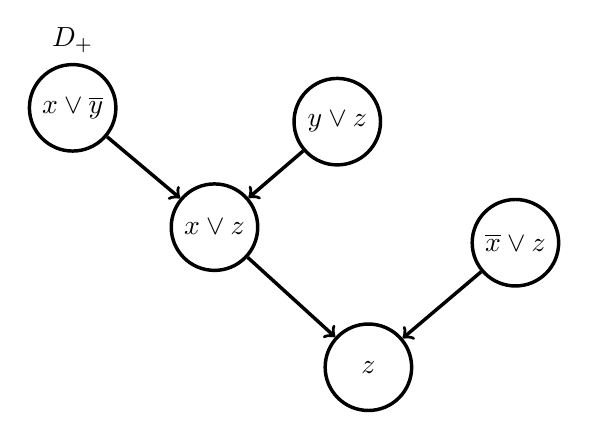
\begin{tikzpicture}
            [every node/.style={inner sep=0pt}]
                \node (1) [circle, minimum size=31.25pt, fill=white, line width=1.25pt, draw=black] at (51.25pt, -49.375pt) {\textcolor{black}{$x \lor \overline{y}$}};
                \node (2) [circle, minimum size=31.25pt, fill=white, line width=1.25pt, draw=black] at (102.5pt, -92.5pt) {\textcolor{black}{$x \lor z$}};
                \node (3) [circle, minimum size=31.25pt, fill=white, line width=1.25pt, draw=black] at (146.875pt, -54.375pt) {\textcolor{black}{$y \lor z$}};
                \node (4) [circle, minimum size=31.25pt, fill=white, line width=1.25pt, draw=black] at (211.25pt, -98.125pt) {\textcolor{black}{$\overline{x} \lor z$}};
                \node (5) [circle, minimum size=31.25pt, fill=white, line width=1.25pt, draw=black] at (158.125pt, -143.125pt) {\textcolor{black}{$z$}};
                \draw [line width=1.25, ->, color=black] (1) to  (2);
                \draw [line width=1.25, ->, color=black] (3) to  (2);
                \draw [line width=1.25, ->, color=black] (2) to  (5);
                \draw [line width=1.25, ->, color=black] (4) to  (5);
                \node at (51.25pt, -25.0pt) {\textcolor{black}{$D_+$}};
            \end{tikzpicture}
        \end{center}

        \begin{center}

            \begin{tikzpicture}
            [every node/.style={inner sep=0pt}]
                \node (1) [circle, minimum size=31.25pt, fill=white, line width=1.25pt, draw=black] at (51.25pt, -49.375pt) {\textcolor{black}{$x \lor \overline{y}$}};
                \node (2) [circle, minimum size=31.25pt, fill=white, line width=1.25pt, draw=black] at (102.5pt, -92.5pt) {\textcolor{black}{$x$}};
                \node (3) [circle, minimum size=31.25pt, fill=white, line width=1.25pt, draw=black] at (146.875pt, -54.375pt) {\textcolor{black}{$y$}};
                \node (4) [circle, minimum size=31.25pt, fill=white, line width=1.25pt, draw=black] at (211.25pt, -98.125pt) {\textcolor{black}{$\overline{x}$}};
                \node (5) [circle, minimum size=31.25pt, fill=white, line width=1.25pt, draw=black] at (158.125pt, -143.125pt) {\textcolor{black}{$0$}};
                \draw [line width=1.25, ->, color=black] (1) to  (2);
                \draw [line width=1.25, ->, color=black] (3) to  (2);
                \draw [line width=1.25, ->, color=black] (2) to  (5);
                \draw [line width=1.25, ->, color=black] (4) to  (5);
                \node at (51.25pt, -25.0pt) {\textcolor{black}{$D_-^{\textrm{без z}}$}};
            \end{tikzpicture}
        \end{center}

        \begin{center}

            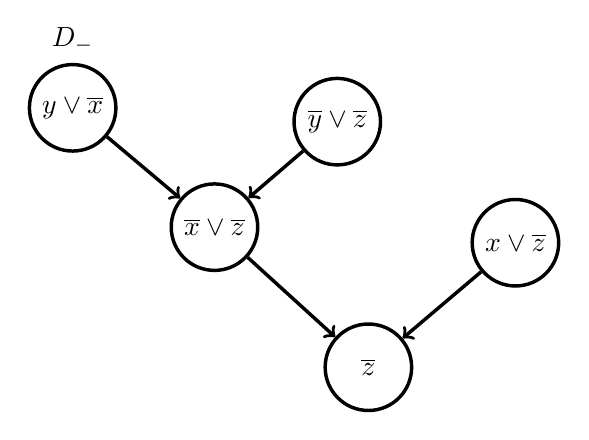
\begin{tikzpicture}
            [every node/.style={inner sep=0pt}]
                \node (1) [circle, minimum size=31.25pt, fill=white, line width=1.25pt, draw=black] at (51.25pt, -49.375pt) {\textcolor{black}{$y \lor \overline{x}$}};
                \node (2) [circle, minimum size=31.25pt, fill=white, line width=1.25pt, draw=black] at (102.5pt, -92.5pt) {\textcolor{black}{$\overline{x} \lor \overline{z}$}};
                \node (3) [circle, minimum size=31.25pt, fill=white, line width=1.25pt, draw=black] at (146.875pt, -54.375pt) {\textcolor{black}{$\overline{y} \lor \overline{z}$}};
                \node (4) [circle, minimum size=31.25pt, fill=white, line width=1.25pt, draw=black] at (211.25pt, -98.125pt) {\textcolor{black}{$x \lor \overline{z}$}};
                \node (5) [circle, minimum size=31.25pt, fill=white, line width=1.25pt, draw=black] at (158.125pt, -143.125pt) {\textcolor{black}{$\overline{z}$}};
                \draw [line width=1.25, ->, color=black] (1) to  (2);
                \draw [line width=1.25, ->, color=black] (3) to  (2);
                \draw [line width=1.25, ->, color=black] (2) to  (5);
                \draw [line width=1.25, ->, color=black] (4) to  (5);
                \node at (51.25pt, -25.0pt) {\textcolor{black}{$D_-$}};
            \end{tikzpicture}
        \end{center}

    \end{example}

    \textbf{Как доказывать?}

    \underline{Способ 1:}

    Методом резолюций, как в теореме.

    $D \: D_- \: D_+$ решаем 2 подзадачи ~-- не эффективно

    \begin{tikzpicture}
    [every node/.style={inner sep=0pt}]
        \node (1) [circle, minimum size=31.25pt, fill=white, line width=1.25pt, draw=black] at (45.0pt, -163.75pt) {\textcolor{black}{10 пер.}};
        \node (2) [circle, minimum size=31.25pt, fill=white, line width=1.25pt, draw=black] at (103.75pt, -111.25pt) {\textcolor{black}{9пер.}};
        \node (3) [circle, minimum size=31.25pt, fill=white, line width=1.25pt, draw=black] at (108.75pt, -205.625pt) {\textcolor{black}{9пер.}};
        \node (4) [circle, minimum size=31.25pt, fill=white, line width=1.25pt, draw=black] at (168.125pt, -65.0pt) {\textcolor{black}{8пер.}};
        \node (5) [circle, minimum size=31.25pt, fill=white, line width=1.25pt, draw=black] at (171.25pt, -130.625pt) {\textcolor{black}{8пер.}};
        \node (6) [circle, minimum size=31.25pt, fill=white, line width=1.25pt, draw=black] at (170.625pt, -176.25pt) {\textcolor{black}{8пер.}};
        \node (7) [circle, minimum size=31.25pt, fill=white, line width=1.25pt, draw=black] at (170.625pt, -240.0pt) {\textcolor{black}{8пер.}};
        \node (8) [circle, minimum size=31.25pt, fill=white, line width=1.25pt, draw=black] at (236.875pt, -215.625pt) {\textcolor{black}{7пер.}};
        \node (9) [circle, minimum size=31.25pt, fill=white, line width=1.25pt, draw=black] at (236.875pt, -264.375pt) {\textcolor{black}{7пер.}};
        \draw [line width=1.25, ->, color=black] (1) to  (2);
        \draw [line width=1.25, ->, color=black] (2) to  (4);
        \draw [line width=1.25, ->, color=black] (2) to  (5);
        \draw [line width=1.25, ->, color=black] (1) to  (3);
        \draw [line width=1.25, ->, color=black] (3) to  (6);
        \draw [line width=1.25, ->, color=black] (3) to  (7);
        \draw [line width=1.25, ->, color=black] (7) to  (8);
        \draw [line width=1.25, ->, color=black] (7) to  (9);
    \end{tikzpicture}

    и так далее... Всего их будет 512 штук.

    \underline{Способ 2:}
    насыщение по уровням

    Каждый с 0

    \begin{enumerate}
        \item с каждым слагаемым
        \item каждый с исходным шагом
    \end{enumerate}

    \subsection{Исчисление предикатов}

    \begin{definition}
        Формула исчисления предикатов

        \begin{enumerate}
            \item{
                Вводим множество $\sum_f$ ~-- множество функций символов
            }
            \item{
                Вводим множество $\sum_c$ ~-- множество констант (не обязательно функции от 0 переменных)
            }
            \item{
                Вводим множество $\sum_p$ ~-- предикатные символы $P(x)$
            }
            \item{
                Вводим множество предикатных переменных $\sum_x$
            }
        \end{enumerate}

        \textbf{Термины:}

        \begin{enumerate}
            \item $x$ ~-- переменная
            \item{
                $f$ ~-- символ $(f(t_1, \dots t_n))$ ~-- где $t_1, \dots t_n$ ~-- термины
            }
        \end{enumerate}
    \end{definition}


    \begin{definition}

        Логическая формула ~-- функция исчисления предикатов. Выраженте из логических связок, атомарных формул.

        \end{definition}


    $P(x) \lor Q(x,f(y))$ \qquad $P(x) \Rightarrow (Q(x) \lor R(x))$

    Если P - формула, то $\forall x$ P - тоже

    x - переменная $\exists x P$ - тоже

    Наличие переменной внутри P недопустимо.

    \begin{remark}

        Приоритеты связок - смотрите раньше, кванторы имеют максимальный приоритет.

        \end{remark}

    \begin{example}

        $\forall P(x)$

        $\exists x Q(x,y)$

        $\forall x \exists y P(x,y)$

        $\forall x P(x) \Rightarrow \exists x Q(x)$

        $\forall x (P(x) \Rightarrow \exists y Q(y))$

        $\forall x \exists y P(x)$

        $\forall x (P(x)) \Rightarrow \exists x Q(x))$ ~-- не подойдет так как х встречается два раза

        \end{example}

    \begin{definition}

        $\forall x P(x)$ ~-- связное вхождение x в формулу

        \end{definition}

    Если квантора для переменой нет, то это не связное вхождение

    $\forall x P(x,y) \lor \exists y Q(x,y,z)$, где $\forall x P(x $ - связное, y ) - не связное

    $\exists E y Q(y,$ соответсвенное связное)

    $z - $ свободная переменная

    (все вхождения не связаны)

    \textbf{Напоминание}

    Сигнатура ~-- символы для предикатов, функций, константы

    \begin{example}

        P(-,-) f(-) g(-,-) c

        \end{example}

    Определив сигнатуру, используют в формулах только эти символы

    $\exists x \forall y P(x,y) \exists Q(x)$ ~-- не из этой сигнатуры

    \begin{definition}

        Интерпретация

        1) М ~-- предикатное множество

        2) Каждой функциональный символ становится функцией

        f : $M^{k} \rightarrow M$, где k ~-- аргументы f

        \end{definition}

    3) Каждый предикатный символ становится функцией из $M^{k}$ : \{ 0,1 \}

    \begin{example}

        $\forall x P(x) = 0 $ - ложь для Z, P ~-- четное

        $\forall x P(x) = 1$ для Z P(x) : $x^{2} \neq 0 $

        $\forall x \exists y P(x,y) = 1 ZP:x>y$, если = 0 N


        \end{example}

    Для любого числа x найдется число y, такое что x>y

    Вычисление значения формулы в заданной итерации

    1) нужно выбрать значение несвязных переменных

    $\qquad \qquad \qquad y = 10 = 1$

    $\exists x P(x,y) = $

    $\qquad \qquad \qquad y = 0 = 0$

    2) f - функциональный символ f($x_{1} \dots x_{n}$) ~-- считаем как функцию $\Rightarrow$ вычислим все термы

    P ~-- предыдущий символ $P(t_{1} \dots t_{k})$ ~-- считаем сами функцию, получаем 0 или 1

    Логические связки ~-- нужно вычислить внутренню часть для всех x $\in $ M

    $\forall x_{ \dots \dots \dots }$ Всегда 1, значит ответ 1, если хотя бы раз 0, то и общий ответ 0

    $\exists x_{ \dots }$ Надо вычислить внутреннюю часть для всех х

    Если хотя бы 1 раз есть 1, то ответ 1

    Если всегда 0, то ответ 0

    M = N

    P(x) = 1 или х четное \qquad \qquad P(x) = x - четное

    \begin{table}[h!]
                \centering
                \begin{tabular}{|c|c|}
                    \hline
                    $\forall x$ & $P(x)$ \\ \hline
                    1      & 1       \\ \hline
                    2      & 0       \\ \hline
                    3      & 1       \\ \hline
                    .      & .       \\ \hline
                    .      & .       \\ \hline
                    .      & .       \\ \hline
                \end{tabular}
            \end{table}

    $\Rightarrow \forall x P(x) = 0$

    $\exists x P(x)$ в той же интерпретации

    \begin{table}[h!]
                \centering
                \begin{tabular}{|c|c|}
                    \hline
                    $\forall x $ & $P(x)$ \\ \hline
                    1      & 1       \\ \hline
                    2      & 0       \\ \hline
                    3      & 1       \\ \hline
                    .      & .       \\ \hline
                    .      & .       \\ \hline
                    .      & .       \\ \hline
                \end{tabular}
            \end{table}

    $\exists x P(x) = 1$

    \begin{example}

        $\forall x \exists y P(x,y) $ \qquad $M = N$ \qquad $P(x,y) : x > y$

        \textbf{x = 1}

        \begin{table}[h!]
                \centering
                \begin{tabular}{|c|c|}
                    \hline
                    $ y $ & $P(x,y)$ \\ \hline
                    1      & 0       \\ \hline
                    2      & 0       \\ \hline
                    3      & 0       \\ \hline
                    4      & 0       \\ \hline
                    5      & 0       \\ \hline
                    .      & .       \\ \hline
                    .      & .       \\ \hline
                \end{tabular}
            \end{table}

        \textbf{x = 2}

        \begin{table}[h!]
                \centering
                \begin{tabular}{|c|c|}
                    \hline
                    $ y $ & $P(x,y)$ \\ \hline
                    1      & 1       \\ \hline
                    2      & 0       \\ \hline
                    3      & 0       \\ \hline
                    4      & 0       \\ \hline
                    5      & 0       \\ \hline
                    .      & .       \\ \hline
                    .      & .       \\ \hline
                \end{tabular}
            \end{table}

        \textbf{x = 3}

        \begin{table}[h!]
                \centering
                \begin{tabular}{|c|c|}
                    \hline
                    $ y $ & $P(x,y)$ \\ \hline
                    1      & 1       \\ \hline
                    2      & 1       \\ \hline
                    3      & 0       \\ \hline
                    4      & 0       \\ \hline
                    5      & 0       \\ \hline
                    .      & .       \\ \hline
                    .      & .       \\ \hline
                \end{tabular}
            \end{table}

        $\exists y P(x,y)$ Вычисляем для $\forall y P(x,y)$

        $\forall x \exists y P(x,y) = 0$ при x = 1



        \end{example}

    \begin{example}

        В той же интерпретации $\exists y \forall x P(x,y)$

        \begin{table}[h!]
                \centering
                \begin{tabular}{|c|c|}
                    \hline
                    $\forall x $ & $P(x)$ \\ \hline
                    y = 1      & 0       \\ \hline
                    y = 2      & 0       \\ \hline
                    y = 3      & 0       \\ \hline
                    .      & .       \\ \hline
                    .      & .       \\ \hline
                    .      & .       \\ \hline
                \end{tabular}
            \end{table}

        \begin{remark}

            Часто функциональные символы, кванторы, пишут "привычно"

            \end{remark}

        $\forall x P(f(x),x)$

        Если P(x,y) = x > y, то будет $\forall x (x + 1 > x)$

        f(x) = x + 1

        Префиксная форма

        инфиксная форма

        \end{example}

    \begin{example}

        Все люди смертны 1

        сократ человек 2

        сократ смертен 3

        \end{example}

    M = \{ Все живые существа\}

    H(x) ~-- x - человек

    S ~-- константы S $\in$ M, S ~-- сократ

    P(x) ~-- смертен

    $H(s)_{2} * \forall x [ h(x) \Rightarrow P(x)  ]_{1} \Rightarrow D(s)_{3}$

    Эта формула истинна, но:

    Возьмем интерпретацию и сигнатуру M = N, предикаты =, >. ф - символ +

    $\exists K (x + k) = y$ - x,y свободные

    x = 5 \qquad y = 10 \quad 1

    x = 10 \qquad y = 5 \quad 0

    $\exists x (x+k=y) = x <y$

    $\forall (x < k \lor x = k) = x = 1$

    $\forall k (\exists t(x+t=k) \lor x = k) =x = 1 $


    \textbf{Напоминание}

    Что такое функция исчисления предикатов

    $\forall x (\exists y P(f(x), y) \lor Q(g(x, c)))$

    $f, g, c$ ~-- функции

    $(f(x), y), (g(x, c))$ ~-- атамарные формы

    $x, f(x), (f(x),y), x, c, g(x, c)$ ~-- термы

    $P, Q$ ~-- предикаты

    $\forall \quad \exists$ ~-- кванторы

    \begin{definition}
        Сигнатура ~-- это множество функциональных символов и предикатов

        $${ f^1, g^2, e^0, P^2, Q^1}$$
    \end{definition}

    \begin{definition}
        Интерпретация ~-- множество + смысл предикатов и функций
    \end{definition}

    В интерпретации функция ~-- это предикат от несвязных переменных


    $\forall x (x \geq x)$ ~-- все переменные связаны = 1

    $\forall (x \geq y)$ ~-- y не связанная переменная $=$
    $\left \{
    \begin{gathered}
        1 \quad y = 1  \\
        0 \quad y \neq 1 \\
    \end{gathered}
    \right.$

    в $M = \mathbb{N}$


    \begin{example}
        $M = \mathbb{N} = { 1, 2, 3, \dots}$ функции  $= +$

        $x > y = \exists k (x = y + k)$

        $x \geq y = x > y \lor x = y = \exists k (x = y + k)  \lor x = y$

        $x$ ~-- четные $= \exists k (x = k + k)$

        $x = 1 \quad = \forall y (y \geq x) = \forall y (\exists k (y = x + k) \lor y = x)$

        Добавим в функции $\cdot$

        $x \vdots y =  \exists k (x = y \cdot k)$

        $x \in \mathbb{P}$ ~-- простое число $= \overline{\exists y [(x \vdots y) \cdot (y > 1) \cdot (y < x)]} (x > 1) = $

        $= \forall y (x \vdots y \Rightarrow y = x \lor y = 1) (x > 1)$

    \end{example}

    \begin{definition}
        Пусть $F, G$ ~-- функции исчисления предикатов

        $F$ ~-- тождественно равно $G (F = G)$, если их значения совпадают в $\forall$ интерпретации
    \end{definition}

    \begin{example}
        $\forall x (P(x) \Rightarrow Q(x)) = \forall x (\overline{P(x)} \lor Q(x))$

        $F = G$

        Данные функции тоже равны $a \Rightarrow b = \overline{a} \lor b$
    \end{example}

    \begin{remark}
        Если функции отличаются заменой, верной в логике исчислений высказываний, то они равны
    \end{remark}

    \begin{example}
        $\overline{\exists x P(x) \lor \exists x Q(x)} = \overline{\exists x P(x)} \cdot \overline{\exists x Q(x)}$
    \end{example}

    \subsubsection{Операции преобразования}

    \begin{enumerate}

        \item{
            Переименование переменной, если $P$ не содержит $y$

            $\forall x P(x) = \forall y P(y) \qquad \exists x P(x) = \exists y P(y)$

            $\exists k (x = y + k) = \exists l (x = y + l) \neq \exists x (x = y + x) \neq \exists y (x = y + y)$

            $\exists x \forall y P(x, y) = \exists x \forall z P (x, z) \neq \exists x \forall x P(x, x)$ ~-- некорректная функция
        }

        \item{
            $\forall x \forall y P(x, y) = \forall y \forall x P(x, y)$

            $\exists x \exists y P(x, y) = \exists y \exists x P(x, y)$


            \textbf{Доказательство для $\forall$}

            Рассмотрим интерпретацию $I$

            левая функция истанна $\Leftrightarrow P(x, y) = 1 \quad \forall x, y \in M$

            Правая функция истинна $\Leftrightarrow P(x, y) = 1 \quad \forall x, y \in M$

            \begin{remark}
                $\exists x \forall y P(x, y) \neq \forall y \exists x P(x, y)$

                $I M = \mathbb{R}, P(x, y): x > y$

                $\forall y \exists x (x > y) = 1$

                $\exists x \forall y (x > y) = 0$
            \end{remark}
        }

        \item{
            $\overline{\forall x P(x)} = \exists x \overline{P(x)}$

            $\overline{\exists x P(x)} = \forall x \overline{P(x)}$

            \textbf{Доказательство для $\forall$}

            $I M, P M \rightarrow \{ 0, 1\}$

            Если слева 0

            $\overline{\forall x P(x)} = 0 \Leftrightarrow \forall x P(x) = 1$

            $\Leftrightarrow P(x) = 1, x \in M$

            $\Leftrightarrow \overline{P(x)} = 0, x \in M$

            $\Leftrightarrow \exists x \overline{P(x)} = 0$
        }

        \item{
            $\exists x P(x) \lor \exists x Q(x) = \exists x (P(x) \lor Q(x))$

            $\forall x P(x) \cdot \forall x Q(x) = \forall x (P(x) \cdot Q(x))$

            \textbf{Доказательство для $\exists$}

            Возьмем $I M, P \mathbb{R}$



            слева $ = 0 \Leftrightarrow$
            $\left \{
            \begin{gathered}
                \exists x P(x) = 0 \\
                \exists x Q(x) = 0 \\
            \end{gathered}
            \right.$
            $\Leftrightarrow$
            $\left \{
            \begin{gathered}
                P(x) = 0, x \in M \\
                Q(x) = 0, x \in M \\
            \end{gathered}
            \right.$
            $\Leftrightarrow P(x) \lor Q(x) = 0, x \in M \Leftrightarrow$

            $\exists x (P(x) \lor Qx()) = 0$

            аналогично для $\forall$

            \begin{remark}
                Для другой связки

                $\forall x P(x) \lor \forall x Q(x) \neq \forall x (P(x) \lor Q(x))$

                Рассмотрим $I: M = \mathbb{N}$

                $P(x)$ ~-- x четные

                $Q(x)$ ~-- x нечетные

                $\forall x P(x) = 0$

                $\forall x Q(x) = 0$

                $\forall x P(x) \lor \forall x Q(x) = 0 \lor 0 = 0$

                $\forall x (P(x) \lor Q(x)) = 1$
            \end{remark}

        }

        \item{
            похожа на 4

            $\exists x P(x) \cdot Q = \exists x (P(x) \cdot Q)$

            $\exists x P(x) \lor Q = \exists x (P(x) \lor Q)$

            $\forall P(x) \cdot Q = \forall x (P(x) \cdot Q)$

            $\forall x P(x) \lor Q = \forall x (P(x) \lor Q)$

            \textbf{Доказательство}

            $I: M, P, Q$

            $a \in M$

            слева 1 $\Leftrightarrow$
            $\left \{
            \begin{gathered}
                \exists x P(x) = 1 \\
                Q = 1 \\
            \end{gathered}
            \right.$
            $\Rightarrow$
            $\left \{
            \begin{gathered}
                P(a) = 1 \\
                Q = 1 \\
            \end{gathered}
            \right.$
            $\Rightarrow P(a) \cdot Q = 1$

            $\Rightarrow \exists x (P(x) \cdot Q) = 1$

            Если слева 0

            если $Q = 0 \Rightarrow P(x) \cdot Q = \exists x (P(x) \cdot Q) = 0$

            если $Q = 1 \Rightarrow$

            $\exists x P(x) = 0 $

            $\Rightarrow P(x) = 0, x \in M$

            $\Rightarrow P(x) \cdot Q = Q, x \in M $

            $\Rightarrow \exists x (P(x) \cdot Q) = 0$

        }

        \item{
            $\exists x P = P$

            $\forall x P = P$

            \begin{example}
                $\forall x P(x, f(x)) \Rightarrow Q$

                $\exists w (\forall x P(x, f(x)) \Rightarrow Q)$
            \end{example}
        }

    \end{enumerate}

    \subsubsection{Нормальные формы}

    \textbf{Мн Ж, КНФ, ДНФ}

    \begin{definition}
        Предваренная нормальная форма

        Формула исчисления предикатов имеет ПНФ, если

        $$Q_1 x_1 Q_2 x_2 \dots Q_n x_n (  Matrix  )$$

        $Q_i = \forall$ или $\exists$

        Простыми словами, ПНФ ~-- это когда все кванторы стоят впереди
    \end{definition}

    \begin{example}
        $\forall x \exists y (P(x, y) \Rightarrow Q(y))$
    \end{example}

    \begin{example}
        $\forall x (P(x, y, z) \lor Q(c))$
    \end{example}

    \begin{example}
        $\cancel{\forall x P(x) \cdot \exists x Q(x)}$
    \end{example}

    \begin{example}
        $\cancel{\forall x (\exists y P(y) \lor Q(x))}  = \forall x \exists y (P(y) \lor Q(x))$
    \end{example}


    \begin{theorem}
        Любая формула исчисления предикатов имеет ПНФ
    \end{theorem}

    \textbf{Алгоритм приведения}

    \begin{enumerate}
        \item{
            Все связки кроме $\&, \lor, \neg$ заменяются на $\&, \lor, \neg$

            $a \Rightarrow b = \overline{x} \lor b$

            $a \Leftrightarrow b = (a \lor \overline{b})(\overline{a} \lor b)$
        }

        \item{
            Все отрицания внутри кванторов

            $\overline{\forall x P(x)} = \exists x \overline{P(x)}$

            $\overline{\exists x P(x)} = \forall x \overline{P(x)}$
        }

        \item{
            По свойству 6 вынести все кванторы в начало, возможно, заменной переменных
        }
    \end{enumerate}


    \begin{example}
        $\forall x P(x) \lor \forall x Q(x)$

        $\neq \forall x (P(x) \lor Q(x))$

        $ = \forall x P(x) \lor \forall y Q(y) = $

        $= \forall x (P(x) \lor \forall y Q(y)) = $

        $= \forall x \forall y (P(x) \lor Q(y))$ ~-- ПНФ
    \end{example}


    \subsubsection{Предваренная нормальная форма}

    \begin{example}

        1) $\forall x P(x) \Rightarrow \exists x Q(x) = \overline{\forall x P(x)} \lor \exists x Q(x)
        = \exists x P(x) \lor \exists x Q(x) = \exists x
        ( P(x) \lor Q(x))$

    \quad ПНФ

        2) $\exists x \overline{P(x)} \lor \exists y Q(y) = \exists x (\overline{P(x)} \lor \exists y Q(y)) =
        \exists x \exists y (\overline{P(x)} \lor Q(x))$

    \qquad \qquad \qquad \qquad \qquad \qquad \qquad \qquad \qquad \qquad \qquad ПНФ

        Результаты 1) и 2) эквивалетные

    \end{example}

    \subsubsection{Сколемовская нормальная форма}

    \begin{definition}
        ПНФ, где $\forall \dots \forall (\dots)$

        \qquad \qquad \qquad \qquad \qquad \quad $\uparrow$ \qquad \quad $\uparrow$

        \qquad \quad  только квантеры $\forall$ \qquad КНФ

        \qquad \qquad \qquad нет $\exists$


        \end{definition}

    \begin{example}

        $\forall x \forall y [ (P(x) \lor \overline{Q(x,y)}(R(x) \lor P(y)))]$

        нет $\exists$ в [ ] КНФ

        \end{example}

    \begin{example}

        $\forall x \forall y (P(x) \lor Q(x)R(y)) = \forall x \forall y [(P(x) \lor Q(x))(P(x) \lor R(y))]$

        \qquad \qquad \qquad \qquad не КНФ \qquad \qquad \qquad \qquad \qquad \qquad КНФ

        $\Rightarrow $ получили СНФ


        \end{example}

    \begin{definition}

        Сколемизация - действие по избавлению от $\exists$ в ПНФ.

        \end{definition}

    Действует так:

    $\forall x_{1} \forall x_{2} \exists x_{3} \forall x_{4} \exists x_{5} \forall x_{6} P(x_{1};x_{2};
    x_{3};x_{4};x_{5};x_{6}) \rightarrow^{CK}$
    
    $ \forall x_{1} \forall x_{2} \forall x_{3} \forall x_{4} \forall x_{5}
    \forall x_{6} P(x_{1};x_{2};f(x_{1};x_{2});x_{4};g(x_{1};x_{2};x_{4});x_{6})$

    $f(x_{1};x_{2})$ ~-- новый функциональный символ


    Убираем $\exists$, все вхождения переменной x заменяются на f(...)


    f(все переменные до $\exists$)

    f ~-- новый функциональный символ


    \begin{example}

        $\exists x \forall y [P(x,y) \lor Q(x,y)] \rightarrow^{CK} \forall y [P(c,y) \lor Q(c,y)]$

        \begin{remark}

            Сколемизация не создает эквивалетную формулу

            \end{remark}

        $\exists x f(x) \rightarrow^{CK} P(c)$

        В интерпретации

        M = N \quad P(x) - четные

        $\exists x P(x) = 1 \neq P(c) = 0 \Rightarrow^{CK} P(c) * \overline{P(c)} = 0 $

        \begin{theorem}

        При сколемизации выполнимые формулы остаются выполнимыми и наоборот

        \end{theorem}

    \begin{example}

        $\exists x (P(x) * \overline{P(x)}) = 0 $

        \end{example}


        Чего не хватает для метода резолюций в исчислении предикатов


        Задача:

        $P_{1} = $ все люди смертны

        $P_{2} = $ сократ человек

        М - все предметы

        Q = сократ смертен

        $P_{1} = \forall x (H(x) \Rightarrow M(x))$

        $H(x) $ - человек

        $M(x)$ - смертен

        $P_2$ = H (сократ) \quad \quad сократ - const $\in$ M

        $P_{1} * P_{2} * \overline{Q}$

        $P_{i}Q$ - в СНФ

        $P_{1} = \forall x (\overline{H(x)} \lor M(x))$

        $P_{2} = $ H (сократ)

        $\overline{Q} = \overline{M(сократ)})$

        Дизъюнкты: $\overline{H(x)} \lor M(x);$ H(сократ); $\overline{M(\textrm{сократ})}$

        \qquad \qquad \qquad $\bar{A} \lor B$ \qquad \qquad $C$ \qquad \qquad $\bar{D}$

        \end{example}

    $\overline{H(x)} \lor M(x)| x = $ сократ

    В методе резолюций для исчисления предикатов необходимо делать подстановки в переменные.

    Отступление про унификацию:

    \begin{definition}

        Сделать подстановку, чтобы формулы стали одинаковыми

        \end{definition}

    P(x,c) \qquad \qquad \qquad P(f(y,c))

    $\searrow \qquad  x = f(c) \qquad \swarrow$

    $ \qquad \searrow  y = c \qquad \swarrow$

    \qquad \qquad P(f(c),c)

    \begin{example}

        \textbf{метода резолюций}

        M ~-- люди из компании

        P(x,y) ~-- x знаком c y.

\usetikzlibrary{shapes.geometric}
\begin{tikzpicture}
[every node/.style={inner sep=0pt}]
\node (1) [circle, minimum size=12.5pt, fill=white, line width=0.625pt, draw=black] at (85.625pt, -173.125pt)  {};
\node (2) [circle, minimum size=12.5pt, fill=white, line width=0.625pt, draw=black] at (136.25pt, -237.5pt)  {};
\node (3) [circle, minimum size=12.5pt, fill=white, line width=0.625pt, draw=black] at (286.875pt, -275.625pt)  {};
\node (4) [circle, minimum size=12.5pt, fill=white, line width=0.625pt, draw=black] at (285.625pt, -145.0pt)  {};
\node (5) [circle, minimum size=12.5pt, fill=white, line width=0.625pt, draw=black] at (180.625pt, -97.5pt)  {};
\draw [line width=0.625, color=black] (1) to  [in=209, out=45] (5);
\draw [line width=0.625, color=black] (5) to  [in=131, out=0] (4);
\draw [line width=0.625, color=black] (4) to  [in=45, out=197] (2);
\draw [line width=0.625, color=black] (4) to  [in=61, out=299] (3);
\end{tikzpicture}

        1) $\forall x P(x,x)$

        2) $\forall x \forall y (P(x,y) \Leftrightarrow P(y,x))$

        \sout{3) $\exists x \exists y P(x,y)$}

        4) $\forall x \forall y \forall z [P(x,y)P(y,z) \Rightarrow P(x,z)]$

        5) $\forall x \forall y \forall z [\overline{P(x,y)} * \overline{(P(y,z)}) \Rightarrow \overline{P(x,z)}]$

        6) $\exists x B(x)$ ~-- существуют мальчики

        7) $\exists x G(x)$ ~-- существуют девочки

        8) $\forall x (B(x) + G(x))$

        9) $\exists x \exists y (B(x)G(y)P(x,y))$

        10) Q: $\forall x \forall y P(x,y)$

        \end{example}

        \begin{example}

            W(x,y) ~-- x может победить y

            1) $\exists x O(x)$ ~-- оборотни существуют

            2) $\exists x G(x)$ ~-- привидения существуют

            3) $\exists x (G(x) \forall y (O(y) \Rightarrow W(x,y) )))$ ~-- есть приведение, которое сильнее всех оборотней

            4) $\exists x V(x)$ ~-- существует вампир

            5) $\forall x \forall y (V(x)G(y) \Rightarrow W(x,y) )$ \quad $\forall $ вампир сильнее $\forall $ приведения

            6) $\overline{ \exists x (V(x) O(x))} $ O не бывает оборотней - вампиров

            0') $\forall x \forall y [\overline{w(x,y)} \lor \overline{w(y,x)}]$

            1') O(o)

            2') G(g)

            3') $\exists x \forall y [G(x)(\overline{(O(y)})) \lor W(x,y)] \rightarrow^{CK} \forall y [ G(\stackrel{ * }{g}) (\overline{O(y)} \lor W(\stackrel{ * }{g},g )) ] $

            4') V(v)

            5') $\forall x \forall y (\overline{V(x)} \lor \overline{G(y)} \lor W(x,y)) $

            6') $\exists x [V(x) O(x)] \rightarrow V(a) o(a) $

            Дизъюнкты: (без $\forall$)

            0) $\overline{w(x,y) } \lor \overline{w(y,x)} $

            1) O(o) 2)G(g) 3) V(v)

            4) $G(\stackrel{ * }{g})$ 5) $\overline{O(y)} \lor W(\stackrel{ * }{g},y) $

            6) $\overline{V(x)} \lor \overline{G(y)} \lor W(x,y)$

            7) V(a)

            8) O(a)



             $
        \left.
        \begin{array}{cc}
            \textcircled{4} y = \stackrel{ * }{g} & \\
            \textcircled{6} &            \\
        \end{array}
        \right. \vline \rightarrow \overline{V(x)} \lor W(x,\stackrel{ * }{g})
        $

            $ $

            9)

             $
        \left.
        \begin{array}{cc}
            \textcircled{9} x= a & \\
            \textcircled{7} &            \\
        \end{array}
        \right. \vline \rightarrow w(a,\stackrel{ * }{g})
        $
            $ $


            10)

                 $
        \left.
        \begin{array}{cc}
            \textcircled{5} y = a & \\
            \textcircled{8} &            \\
        \end{array}
        \right. \vline \rightarrow w(\stackrel{ * }{g},a)
        $

            11)

                   $
        \left.
        \begin{array}{cc}
            \textcircled{0} x = \stackrel{*}{g} & \\
            \textcircled{10} y = a &            \\
        \end{array}
        \right. \vline \rightarrow w(\stackrel{ * }{g},a)
        $

            12)

                     $
        \left.
        \begin{array}{cc}
            \textcircled{11} x = a & \\
            \textcircled{12} y = \stackrel{ * }{g} &            \\
        \end{array}
        \right. \vline \rightarrow \square пустой дизъюнкт
        $
            \end{example}

    \subsubsection{Формальные языки}

    \begin{definition}

        А ~-- Алфавит, любое конечное, не пустое множество

        Обычно, элементы множества обозначаются a,b,c и другими символами

        \end{definition}

    \begin{example}

        A = \{a,b,c\}

        \end{example}

    \begin{definition}

        Слово (предложение) - конечная последовательность элементов алгоритма

        \end{definition}

    \begin{example}

        aa


        bcfbc

        cb

        abcd

        cc

        accaaad

        bab

        c $\rightarrow$ длина 1

       $ \Lambda$ ~-- длина 0 $\Lambda$

        $\Lambda$ ~-- пустое слово




        $\Lambda$ $\notin$ A
        \end{example}

    \begin{definition}

        Язык ~-- это множество слов (предложений)

        \end{definition}

    "Я сплю" $\in$ Русский

    "Я спит" $\notin$ Русский

    "Ябэъъ" $\notin$ Русский

    \begin{example}

        $L_{1} = \{ a,aa,aaa,aaaa, \dots \}$ ~-- язык слов из "a"

        \end{example}

    \begin{example}

        $L_{a} = \{ a,ab,aba,ba,bab \dots \}$ ~-- язык слов из "a и b"

        \end{example}


    \begin{example}
        Язык $L_{a = b} = \{ \textrm{слова, где a и b поровну}\}$

        $abc \in L_{a = b}$

        $abbbcccc \notin L_{a = b}$

        $ababa \notin L_{a = b}$

        $\Lambda \in L_{a = b}$
    \end{example}

    \begin{example}

        $L_{a^n b^n} = \{ a^n b^n \: | n \in \mathbb{N} \cup \{0 \} \} = \{ \Lambda, ab, aabb, aaabbb, \dots \}$

        $x^n$ ~-- повторение $n$ раз

        $L_{a^n b^n} \subset L_{a = b}$
    \end{example}

    \begin{example}
        $A = \{ 0, 1, 2, 3, 4, 5, 6, 7, 8, 9, +, (, ), - \}$

        $L_{tel} = \{ \textrm{язык телефонных номеров} \}$

        $+7 (921) 401-00-00 \in L_{tel}$
    \end{example}

    \begin{definition}
        Грамматика (формальная грамматика) ~-- это формальное описание языка

        Если есть грамматика языка $L$

        $\forall$ слова $w$ можно проверить $w \in L$ ?
    \end{definition}

    \textbf{Типы грамматик:}

    \begin{enumerate}
        \addtocounter{enumi}{-1}
        \item{
            Грамматику можно описать с помощью машины Тьюринга

            Грамматика = программа проверяет $w \in L$ ?

            Если для языка создать программу проверки ~-- это тип 0
        }
        \item{
            Контекстно-зависимые грамматики

            Контекстно-зависимые языки ~-- описываются через конечно-зависимые грамматики
        }
        \item{
            Контекстно-свободные грамматики

            КС языки ~-- те языки, которые можно описать с помощью КС грамматик
        }
        \item{
            Регулярные выражения или конечные автоматы

            Регулярные языки задаются регулярными выражениями или конечными автоматами
        }
    \end{enumerate}

    \begin{remark}
        Каждый следующий вид грамматики "проще предыдущего"

        Но множества его языков сужаются

        Языки типо 0 $\supset$ КЗ-языки $\supset$ КС-языки $\supset$ Регулярные языки
    \end{remark}

    \subsubsection{Машина Тьюринга}

    \begin{definition}
        Машина Тьюринга = ($A; \Box; Q; R; q_0; Q_F$)

        $A$ ~-- алфавит, $\neq \emptyset,$ множество конечное

        $\Box \in A$ ~-- специальный символ

        $Q$ ~-- состояние, $\neq \emptyset,$ множество конечное

        $R$ ~-- правила перехода

        $q_0 \in Q$ ~-- начальное состояние

        $Q_F \subset Q$ ~-- подмножество конечных состояний

        $R: A \times Q \rightarrow A \times Q \times \{ L, R, E - \textrm{не двигаться}\}$
    \end{definition}

    \begin{example}

        $A = \{ 1, \Box \}$

        $Q = \{ q_0, q_1 \}$

        $Q_F = \{ q_1 \}$


        \begin{table}[H]
            \centering
            \begin{tabular}{|c|c|c|}
                \hline
                $R/A$ & 1           & $\Box$      \\ \hline
                $q_0$   & $1, q_1, R$ & $1, q_1, S$ \\ \hline
                $q_1$   & не надо     & не надо     \\ \hline
            \end{tabular}
        \end{table}


        Конечное количество символов ленты $\neq \Box$

        \begin{table}[H]

            \centering
            \begin{tabular}{ *{9}{c} }
                \cline{1-9}
                \multicolumn{1}{|c}{0} &
                \multicolumn{1}{|c}{1} &
                \multicolumn{1}{|c}{2} &
                \multicolumn{1}{|c}{3} &
                \multicolumn{1}{|c}{...} &
                \multicolumn{1}{|c}{...} &
                \multicolumn{1}{|c}{...} &
                \multicolumn{1}{|c}{...} &
                \multicolumn{1}{|c|}{...} \\
                \cline{1-9}
                \cline{1-9}
                \multicolumn{1}{|c}{1} &
                \multicolumn{1}{|c}{1} &
                \multicolumn{1}{|c}{1} &
                \multicolumn{1}{|c}{1} &
                \multicolumn{1}{|c}{$\Box$} &
                \multicolumn{1}{|c}{$\Box$} &
                \multicolumn{1}{|c}{$\Box$} &
                \multicolumn{1}{|c}{$\Box$} &
                \multicolumn{1}{|c|}{...} \\
                \cline{1-9}
                $\uparrow$ \\
                $q_0$
            \end{tabular}
        \end{table}

        Сначало головка смотрит на клетку с индексом 0, состояние $q_0$

        Видим символ 1

        $R(1, q_0) = 1, q_0, R$ ~-- сдвинуть головку вправо

        \begin{table}[H]

            \centering
            \begin{tabular}{ *{9}{c} }
                \cline{1-9}
                \multicolumn{1}{|c}{0} &
                \multicolumn{1}{|c}{1} &
                \multicolumn{1}{|c}{2} &
                \multicolumn{1}{|c}{3} &
                \multicolumn{1}{|c}{...} &
                \multicolumn{1}{|c}{...} &
                \multicolumn{1}{|c}{...} &
                \multicolumn{1}{|c}{...} &
                \multicolumn{1}{|c|}{...} \\
                \cline{1-9}
                \cline{1-9}
                \multicolumn{1}{|c}{1} &
                \multicolumn{1}{|c}{1} &
                \multicolumn{1}{|c}{1} &
                \multicolumn{1}{|c}{1} &
                \multicolumn{1}{|c}{$\Box$} &
                \multicolumn{1}{|c}{$\Box$} &
                \multicolumn{1}{|c}{$\Box$} &
                \multicolumn{1}{|c}{$\Box$} &
                \multicolumn{1}{|c|}{...} \\
                \cline{1-9}
                & $\uparrow$ \\
                & $q_0$
            \end{tabular}
        \end{table}

        Головка на клетке 1

        Символ = 1

        Состояние = $q_0$

        $R(1, q_0) = 1, q_0, R$

        \begin{table}[H]

            \centering
            \begin{tabular}{ *{9}{c} }
                \cline{1-9}
                \multicolumn{1}{|c}{0} &
                \multicolumn{1}{|c}{1} &
                \multicolumn{1}{|c}{2} &
                \multicolumn{1}{|c}{3} &
                \multicolumn{1}{|c}{...} &
                \multicolumn{1}{|c}{...} &
                \multicolumn{1}{|c}{...} &
                \multicolumn{1}{|c}{...} &
                \multicolumn{1}{|c|}{...} \\
                \cline{1-9}
                \cline{1-9}
                \multicolumn{1}{|c}{1} &
                \multicolumn{1}{|c}{1} &
                \multicolumn{1}{|c}{1} &
                \multicolumn{1}{|c}{1} &
                \multicolumn{1}{|c}{$\Box$} &
                \multicolumn{1}{|c}{$\Box$} &
                \multicolumn{1}{|c}{$\Box$} &
                \multicolumn{1}{|c}{$\Box$} &
                \multicolumn{1}{|c|}{...} \\
                \cline{1-9}
                & & $\uparrow$ \\
                & & $q_0$
            \end{tabular}
        \end{table}

        потом

        \begin{table}[H]

            \centering
            \begin{tabular}{ *{9}{c} }
                \cline{1-9}
                \multicolumn{1}{|c}{0} &
                \multicolumn{1}{|c}{1} &
                \multicolumn{1}{|c}{2} &
                \multicolumn{1}{|c}{3} &
                \multicolumn{1}{|c}{...} &
                \multicolumn{1}{|c}{...} &
                \multicolumn{1}{|c}{...} &
                \multicolumn{1}{|c}{...} &
                \multicolumn{1}{|c|}{...} \\
                \cline{1-9}
                \cline{1-9}
                \multicolumn{1}{|c}{1} &
                \multicolumn{1}{|c}{1} &
                \multicolumn{1}{|c}{1} &
                \multicolumn{1}{|c}{1} &
                \multicolumn{1}{|c}{$\Box$} &
                \multicolumn{1}{|c}{$\Box$} &
                \multicolumn{1}{|c}{$\Box$} &
                \multicolumn{1}{|c}{$\Box$} &
                \multicolumn{1}{|c|}{...} \\
                \cline{1-9}
                & & & $\uparrow$
            \end{tabular}
        \end{table}

        потом

        \begin{table}[H]

            \centering
            \begin{tabular}{ *{9}{c} }
                \cline{1-9}
                \multicolumn{1}{|c}{0} &
                \multicolumn{1}{|c}{1} &
                \multicolumn{1}{|c}{2} &
                \multicolumn{1}{|c}{3} &
                \multicolumn{1}{|c}{...} &
                \multicolumn{1}{|c}{...} &
                \multicolumn{1}{|c}{...} &
                \multicolumn{1}{|c}{...} &
                \multicolumn{1}{|c|}{...} \\
                \cline{1-9}
                \cline{1-9}
                \multicolumn{1}{|c}{1} &
                \multicolumn{1}{|c}{1} &
                \multicolumn{1}{|c}{1} &
                \multicolumn{1}{|c}{1} &
                \multicolumn{1}{|c}{$\Box$} &
                \multicolumn{1}{|c}{$\Box$} &
                \multicolumn{1}{|c}{$\Box$} &
                \multicolumn{1}{|c}{$\Box$} &
                \multicolumn{1}{|c|}{...} \\
                \cline{1-9}
                & & & & $\uparrow$
            \end{tabular}
        \end{table}

        Теперь:

        Головка: клетка 4

        Символ: $\Box$

        Состояние: $q_0$

        $R(0, q_0) = 1, q_1, E$ ~-- стоим на месте

        \begin{table}[H]

            \centering
            \begin{tabular}{ *{9}{c} }
                \cline{1-9}
                \multicolumn{1}{|c}{0} &
                \multicolumn{1}{|c}{1} &
                \multicolumn{1}{|c}{2} &
                \multicolumn{1}{|c}{3} &
                \multicolumn{1}{|c}{4} &
                \multicolumn{1}{|c}{...} &
                \multicolumn{1}{|c}{...} &
                \multicolumn{1}{|c}{...} &
                \multicolumn{1}{|c|}{...} \\
                \cline{1-9}
                \cline{1-9}
                \multicolumn{1}{|c}{1} &
                \multicolumn{1}{|c}{1} &
                \multicolumn{1}{|c}{1} &
                \multicolumn{1}{|c}{1} &
                \multicolumn{1}{|c}{1} &
                \multicolumn{1}{|c}{$\Box$} &
                \multicolumn{1}{|c}{$\Box$} &
                \multicolumn{1}{|c}{$\Box$} &
                \multicolumn{1}{|c|}{...} \\
                \cline{1-9}
                & & & & $\uparrow$
            \end{tabular}
        \end{table}

        Дано было 1111, результат 11111

        Вывод: программа дописывает 1

        Работа Машины Тьюринга формально
    \end{example}

    \begin{definition}
        Конфигурация: $(w, n \in \mathbb{N} \cup \{ 0 \}, q)$

        n ~-- положение головки

        $q \in Q$

        $w$ ~-- слово на ленте (без хвоста $\Box$)

        Один шаг исполнения программы:

        $(w_1, n_1, q_1) \rightarrow (w_2, n_2, q_2)$

        $w_1[n_1]$ ~-- символ над головкой

        $R(w_1[n_1], q_1) = (a, q_2, L/R/E)$

        $w_2 = w_1$ где $w_1[n] = a$

        если $L \rightarrow n_2 = n_1 - 1$

        $R \rightarrow n_2 = n_1 + 1$

        $E \rightarrow n_2 = n_1$

        Начало работы: $(w, O, q_0)$

        $w$ ~-- дана

        $O$ ~-- головка слова

        $q_0$ ~-- начальное слово

        $\rightarrow \dots \rightarrow \dots \rightarrow \dots \rightarrow (\overline{\overline{w}}, \overline{q} \in Q_F)$ ~-- конечное состояние

        Ответ: $\overline{\overline{w}}$, то есть из слова $w$ получили $\overline{\overline{w}}$
    \end{definition}

    \begin{remark}
    (Тезис Чёрге)

        Все, что мы интуитивно понимаем как алгоритм, может быть реализовано с помощью машины Тьюринга
    \end{remark}

    \begin{remark}
        Модификации машины Тьюринга:

        \begin{enumerate}
            \item{
                $\infty$ в обе стороны лента
            }
            \item{
                несколько лент
            }
            \item{
                недетерминированная машина Тьюринга
            }
        \end{enumerate}

        1, 2, 3 ~-- это все эквивалент обычной машины Тьюринга
    \end{remark}

    \begin{remark}
        Про проверку, слово в языке? $w \in ? L$

        \begin{table}[H]
            \centering
            \begin{tabular}{ *{9}{c} }
                \cline{1-9}
                \multicolumn{1}{|c}{ } &
                \multicolumn{1}{|c}{ } &
                \multicolumn{1}{|c}{ } &
                \multicolumn{1}{|c}{ } &
                \multicolumn{1}{|c}{ } &
                \multicolumn{1}{|c}{$\Box$} &
                \multicolumn{1}{|c}{$\Box$} &
                \multicolumn{1}{|c}{$\Box$} &
                \multicolumn{1}{|c|}{$\Box$} \\
                \cline{1-9}
            \end{tabular}
        \end{table}

        Если результат $1 \Rightarrow w \in L$

        Если результат $0 \Rightarrow w \notin L$

        или

        $\{ q_1, q_2\} = Q_F$

        $q_1: w \in L$

        $q_2: w \notin L$

        Все зависит от конечного состояния
    \end{remark}

    \subsubsection{Контекстно-свободные языки}

    \begin{example}
        Email @ server

        username $\rightarrow$ word

        server $\rightarrow$ word.word

        word $\rightarrow \frame{a}$

        word $\rightarrow \frame{b}$

        word $\rightarrow \frame{c}$

        $E \rightarrow u@S \rightarrow w@S \rightarrow$ (используя правило $s \rightarrow w.w$) $w@w.w \rightarrow$ (используя правило $w \rightarrow ww$) $ww@w.w$

        $\rightarrow xw@w.w \rightarrow xy@w.w$

        $\rightarrow xy@ww.w \rightarrow xy@www.w$

        $\rightarrow xy@www.ww$
    \end{example}

    Можно ли получить $xy@@ru$?

    нет $\notin L$

    то есть слова, которые можно получить, они $\in L$

    \begin{example}

        Еще

        \begin{enumerate}
            \item{
                $S \rightarrow$
            }
            \item{
                $S \rightarrow aSb$
            }
        \end{enumerate}

        ~-- это грамматика

        $S \rightarrow aSb \rightarrow aaSbb \rightarrow aaaSbbb \rightarrow aaabbb$

        Какие слова можно вывести?

        $\{ a^n b^n | n \geq 0\} = \{ \Lambda, ab, aabb, aaabbb, \dots  \}$
    \end{example}

    \begin{definition}
        КС-грамматика ~-- $(A, N, S \in N, R)$

        $A$ ~-- алфавит терминальных символов ~ конечен, $\neq \emptyset$

        $N$ ~-- алфавит нетерминальных символов, конечен, $\neq \emptyset$

        $S$ ~-- начальный нетерминальный

        $R$ ~-- множество правил
    \end{definition}


	КС ~-- грамматика

	А ~-- Алфавит

	N ~-- нетерминальные символы (алф.)

	S $\in$ N ~-- начальное

	R ~-- правило вида $N \rightarrow (A \lor N)^{*}$

	\begin{definition}

		Из слова $w \in ( A \in N)^{*}$ выводится u $\in (A \lor N)^{*}$ если w = $\dots x \dots \rightarrow u = \dots $ Y $\dots$

		где $X \rightarrow Y \in R$
		\end{definition}

	\begin{definition}

		Вывод ~-- это последовательность $w_{i} : w_{i-1} \rightarrow w_{i}$

		\end{definition}

	$w_{1} \rightarrow w_{2} \rightarrow w_{3} \dots \rightarrow w_{n} = w_{1} \rightarrow^{*} w_{n}$

	вывод $w_{n} $ из $w_{1}$

	\begin{definition}

		Язык, который задает КС - грамматика

		$L = \{ w/ \exists $ вывод $S^{*} \rightarrow w$ $\}$

		\end{definition}

	\begin{example}

		1) HTML \qquad H ~-- начальный нетерминал

		$H \rightarrow EH$ \qquad \qquad \qquad T ~-- тэг, L ~-- символы

		$H \rightarrow$

		$H \rightarrow $

		$H \rightarrow EH$

		$H \rightarrow EH \rightarrow EEH \rightarrow EE$

		$H \rightarrow EE \dots E$

		$E \rightarrow T$

		$E \rightarrow L$

		$L \rightarrow a$

		$L \rightarrow b$

		$L \rightarrow c$

		$.$

		$.$

		$L \rightarrow A$

		\end{example}

	Устройство тэгов:

	$T \rightarrow O$

	Т ~-- тэг

	L ~-- символы

	O ~-- открывание тэга

	С ~-- закрывание тэга

	T ~-- ОНС

	T ~-- $< \dots > \dots <\dots>$

	T ~-- $< \dots >_{img}$

	O $\rightarrow <N>$

	C $\rightarrow <\mathbf{N}>$

	N $\rightarrow$

	N $\rightarrow LN$

	N $\rightarrow$ LLLL

	Выведем hello,<b>World<h>!

	$H \rightarrow EH \rightarrow EEG \rightarrow^{*} EEEEEEEEEH \rightarrow EEEEEEEEE \rightarrow^{*} LLLLLLLTL \rightarrow^{*} h,T!$

	$\rightarrow hello, <N> world <\mathbf{N}>!$

	$\rightarrow^{*} hello, <b> world </b>!$

	Итого, hello, <b> world $</t>! \in \alpha$

	Что есть в теме?

	~-- алгоритм разбора

		Дана грамматика, слово, получить вывод слова или понять, что оно не выводится ~-- специальные виды грамматик с эффектом алг. разбора

	$*LL(1) LR(1) LALR(1) \dots$

	\subsubsection{Регулярные языки}

	Задаются регулярными выражениями и конечными автоматами

	Регулярные языки и выражения

	\begin{definition}

		Регулярные языки

		1) $\{a\}$, где $a \in A$ регулярный

		2) если $L_{1}$ и $L_{2}$ ~-- регулярные, то $L_{1}L_{2} = \{w_{1}w_{2}\}, w_{1} \in L_{1}, w_{2} \in L_{2})$ ~-- регулярный

		$L_{1}L_{2}$ ~-- регулярные

		$L_{1}|L_{2} = L_{1} \lor L_{2}$ ~-- регулярный

		\end{definition}

	\begin{example}

		A = $\{a,b,c\}$

		$\{a\}$ \qquad $\{b\} = \{ad\}$

		$\{ab\}|\{b\}=\{abc\}$

		$\{a\}|\{b\} = \{a,b\}$

		$\{a,b\}|\{b\}|\{c\} = \{ab,bc\}$

		$\{ab,b,c\}\{b,bc\} = \{abb,abbc,bb,bbc,cb,cbc\}$

		$\{a\}^{*} = \{\Lambda,a,aa,aaa,\dots \} $

		$\{a,b\}^{*} = \{\Lambda,a,b,aa,ab,ba,bb,aab,abb,\dots \}$ ~-- слова из a и b

		$\{a,bc\}^{*} = \{\Lambda,a,bc,abc,bca,aa,bcbc,\dots,aabc,abcbcaa \}$

		\end{example}

	\begin{definition}

		Регулярные выражения ~-- это выражение над языками.

		\end{definition}

	1) Определим ~-- конк, 1, итерация

	2)$\{a\} $ ~-- записываются как *

	\begin{example}

		$abc^{*} = \{ ab,abc,abcc,abccc,\dots \}$
		$\uparrow$
		конк
		$\downarrow$
		$a(bc)^{*} = \{ a,abc,abcbc,abcbcbc,\dots\}$

		$(0|1|2)(0|1|2|3|\dots|9):(0|1|2|3|4|5)$

		$(0|1|2|\dots|9)$ ~-- время
		\end{example}

	$A = \{ 0,1,2,\dots 9,:\}$

	23:56 \qquad 29:40??

	Нормальное время

	[0123456789]

	$((0|1)(0|1\dots|9)(20|21|22|23):(0|\dots|5)(0)\dots(9))$

	\begin{example}

	$(a|b)^{*} = \{ \Lambda a,b,ab,aa,bb,ba,\dots,abbaab\dots \}$

		$(ab)^{*} = \{ \Lambda, ab,abab,ababab,\dots \}$

		$a^{*}|b^{*} = \{ \Lambda,a,aa,aaa,aaaa,\dots,b,bb,bbb,bbbb,\dots \}$

		\end{example}

	$\{a^{4}b^{4}/n \in \mathbf{N}$ ~-- не регулярный язык

	\begin{definition}

		Конечные автоматы это $\{ Q,S \subset Q, F \subset Q, E \subset Q x Q x A \lor \{\epsilon\}) \}$

		Q ~-- конечное не пустое множество состояний.

		S ~-- начальное состояние

		F ~-- конечные состояние

		A ~-- алфавит

		E ~-- переходы между состояниями

		$q_{1} \rightarrow^{A,\epsilon } q_{2}$

		\end{definition}
		
		$ $
		
		$ $
		
		Это состояние:
		\usetikzlibrary{shapes.geometric}

\begin{tikzpicture}
[every node/.style={inner sep=0pt}]
\node (1) [circle, minimum size=25.0pt, fill=white, line width=0.625pt, draw=black] at (104.375pt, -54.375pt)  {};
\end{tikzpicture}
		
		Начальное состояние:
		\usetikzlibrary{shapes.geometric}

\begin{tikzpicture}
[every node/.style={inner sep=0pt}]
\node (1) [circle, minimum size=25.0pt, fill=white, line width=0.625pt, draw=red] at (62.5pt, -57.5pt)  {};
\end{tikzpicture}

		$ $
		
		$ $
		
		$ $
    Конечное состояние:
    \usetikzlibrary{shapes.geometric}

\begin{tikzpicture}
[every node/.style={inner sep=0pt}]
\node (1) [circle, minimum size=25.0pt, fill=white, line width=0.625pt, draw=green] at (64.375pt, -110.0pt)  {};
\end{tikzpicture}

$ $

$ $

\usetikzlibrary{shapes.geometric}
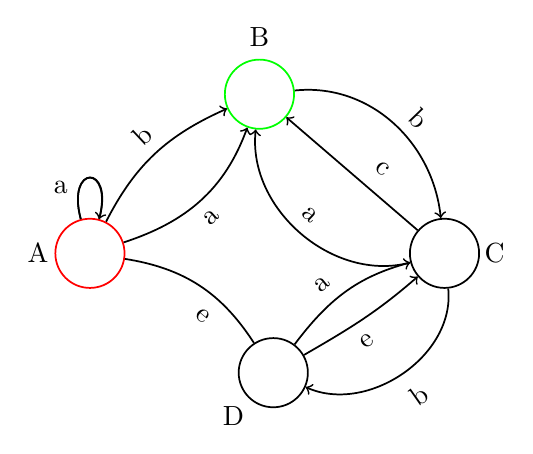
\begin{tikzpicture}
[every node/.style={inner sep=0pt}]
\node (1) [circle, minimum size=25.0pt, fill=white, line width=0.625pt, draw=black] at (110.625pt, -151.25pt)  {};
\node (2) [circle, minimum size=25.0pt, fill=white, line width=0.625pt, draw=black] at (172.5pt, -108.125pt)  {};
\node (4) [circle, minimum size=25.0pt, fill=white, line width=0.625pt, draw=green] at (105.625pt, -50.625pt)  {};
\node (3) [circle, minimum size=25.0pt, fill=white, line width=0.625pt, draw=red] at (44.375pt, -108.125pt)  {};
\draw [line width=0.625, ->, color=black, loop above] (3) to (3);
\draw [line width=0.625, ->, color=black] (3) to  [in=204, out=63] (4);
\draw [line width=0.625, ->, color=black] (3) to  [in=250, out=18] (4);
\draw [line width=0.625, ->, color=black] (4) to  [in=96, out=6] (2);
\draw [line width=0.625, ->, color=black] (2) to  (4);
\draw [line width=0.625, ->, color=black] (2) to  [in=264, out=195] (4);
\draw [line width=0.625, ->, color=black] (1) to  [in=221, out=30] (2);
\draw [line width=0.625, ->, color=black] (1) to  [in=195, out=53] (2);
\draw [line width=0.625, ->, color=black] (2) to  [in=336, out=276] (1);
\draw [line width=0.625, color=black, loop above] (3) to (3);
\draw [line width=0.625, color=black] (3) to  [in=123, out=351] (1);
\node at (96.25pt, -166.875pt) {\textcolor{black}{D}};
\node at (190.625pt, -108.125pt) {\textcolor{black}{C}};
\node at (105.625pt, -30.0pt) {\textcolor{black}{B}};
\node at (25.625pt, -108.125pt) {\textcolor{black}{A}};
\node at (33.75pt, -84.375pt) {\textcolor{black}{a}};
\node at (63.125pt, -65.625pt) [rotate=43] {\textcolor{black}{b}};
\node at (88.125pt, -95.0pt) [rotate=42] {\textcolor{black}{a}};
\node at (163.125pt, -59.375pt) [rotate=314] {\textcolor{black}{b}};
\node at (150.0pt, -77.5pt) [rotate=321] {\textcolor{black}{c}};
\node at (123.75pt, -94.375pt) [rotate=317] {\textcolor{black}{a}};
\node at (144.375pt, -140.0pt) [rotate=34] {\textcolor{black}{e}};
\node at (128.125pt, -119.375pt) [rotate=39] {\textcolor{black}{a}};
\node at (163.125pt, -159.375pt) [rotate=35] {\textcolor{black}{b}};
\node at (85.0pt, -130.625pt) [rotate=320] {\textcolor{black}{e}};
\end{tikzpicture}

	$\epsilon $ ~-- пустой переход

	$Q = \{ A,B,C,D\}$
	
	\begin{definition}
	Конфигурация $\in A^{*} x Q$ ~-- слово и состояние 
	\end{definition}

\begin{example}
(abc,A)
(bb,B)
($\Lambda,A)$
\end{example}

\begin{definition}
Из конфигурации 1 выводится конфигурация 2

$(w_{1}, q_{1}) \rightarrow (w_{2},q_{2})$

если $\exists e \in E: q_{1} \rightarrow^{a} q_{2} $ и $W_{2} = w_{1}a$

\end{definition}

\begin{example}
$(\Lambda,A) \rightarrow (a,A) \rightarrow^{A \rightarrow^{a} A} (aa,A) \rightarrow^{A \rightarrow^{b} B} $

\qquad \qquad $\vdots$

$\rightarrow^{B \rightarrow^{b} c} (aabb,c) \rightarrow^{c \rightarrow^{b} D} (aabbb,D) \rightarrow^{D \rightarrow^{\epsilon} C} (aabbb,c) $

\end{example}

\begin{definition}
Какой язык задает конечный автомат?

слово w $\in$ L, если $\exists $ вывод $(\Lambda,s) \rightarrow \dots \rightarrow (w,f) $, где $s \in S, f \in F$
\end{definition}

S ~-- начальное

f ~-- конечное

если могу прочитать слово w, начав  в начальном состоянии, закончив в конечном.

\begin{definition}
в прошлом примере 

aabbb $\in L$

$aabb \in L$

$aab \in L$

$a \in L$

$a \rightarrow^{\epsilon} D \rightarrow^{a} C $
\end{definition}

\begin{example}

$ $

$ $

$ $
\usetikzlibrary{shapes.geometric}
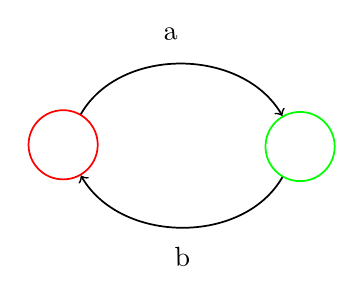
\begin{tikzpicture}
[every node/.style={inner sep=0pt}]
\node (1) [circle, minimum size=25.0pt, fill=white, line width=0.625pt, draw=red] at (64.375pt, -110.625pt)  {};
\node (2) [circle, minimum size=25.0pt, fill=white, line width=0.625pt, draw=green] at (150.0pt, -111.25pt)  {};
\draw [line width=0.625, ->, color=black] (1) to  [in=120, out=60] (2);
\draw [line width=0.625, ->, color=black] (2) to  [in=300, out=240] (1);
\node at (103.125pt, -70.625pt) [rotate=4] {\textcolor{black}{a}};
\node at (107.5pt, -151.25pt) [rotate=1] {\textcolor{black}{b}};
\end{tikzpicture}

L = $\{ a,aba,ababa,\dots \}$ = $a(ba)^{*}$
\end{example}

\textbf{Увтерждение}

Язык регулярный $\Leftrightarrow \exists$ конечный автомат, который его принимает

AB: \textcircled{} $\rightarrow^{A}$ \textcircled{} $\rightarrow^{B}$ B

A/B:

\qquad \quad $ A $

\qquad $\nearrow \searrow$

$\textcircled{} $ \qquad \quad $\textcircled{}$

\qquad $\searrow$  $\nearrow$

\qquad \quad $ B $

$A^{*}$

\usetikzlibrary{shapes.geometric}
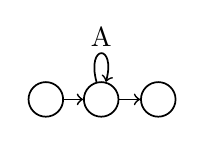
\begin{tikzpicture}
[every node/.style={inner sep=0pt}]
\node (1) [circle, minimum size=12.5pt, fill=white, line width=0.625pt, draw=black] at (85.625pt, -63.125pt)  {};
\node (2) [circle, minimum size=12.5pt, fill=white, line width=0.625pt, draw=black] at (65.0pt, -63.125pt)  {};
\node (3) [circle, minimum size=12.5pt, fill=white, line width=0.625pt, draw=black] at (45.0pt, -63.125pt)  {};
\draw [line width=0.625, ->, color=black] (3) to  (2);
\draw [line width=0.625, ->, color=black] (2) to  (1);
\draw [line width=0.625, ->, color=black, loop above] (2) to (2);
\node at (65.0pt, -40.625pt) {\textcolor{black}{A}};
\end{tikzpicture}

Авт $\rightarrow $ Регулярное выражение - убирание вершин

\begin{definition}
Детерминированный КА ~-- это КА, у которого

1) |S| = 1 ровно 1 нач вершина

2) нет $\epsilon$ ~-- переходов

3) $\textcircled{} \nearrow \searrow$ нет двух переходов с одинаковыми символами и началом
\end{definition}

\usetikzlibrary{shapes.geometric}
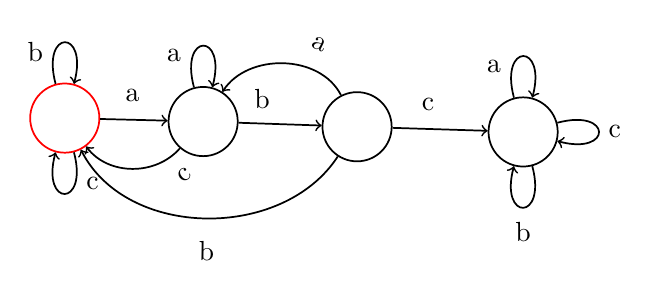
\begin{tikzpicture}
[every node/.style={inner sep=0pt}]
\node (1) [circle, minimum size=25.0pt, fill=white, line width=0.625pt, draw=red] at (26.25pt, -59.375pt)  {};
\node (2) [circle, minimum size=25.0pt, fill=white, line width=0.625pt, draw=black] at (76.25pt, -60.625pt)  {};
\node (3) [circle, minimum size=25.0pt, fill=white, line width=0.625pt, draw=black] at (131.875pt, -62.5pt)  {};
\node (4) [circle, minimum size=25.0pt, fill=white, line width=0.625pt, draw=black] at (191.875pt, -64.375pt)  {};
\draw [line width=0.625, ->, color=black, loop above] (1) to (1);
\draw [line width=0.625, ->, color=black, loop below] (1) to (1);
\draw [line width=0.625, ->, color=black] (1) to  (2);
\draw [line width=0.625, ->, color=black] (2) to  (3);
\draw [line width=0.625, ->, color=black] (3) to  (4);
\draw [line width=0.625, ->, color=black, loop above] (2) to (2);
\draw [line width=0.625, ->, color=black] (3) to  [in=57, out=117] (2);
\draw [line width=0.625, ->, color=black, loop above] (4) to (4);
\draw [line width=0.625, ->, color=black, loop right] (4) to (4);
\draw [line width=0.625, ->, color=black, loop below] (4) to (4);
\draw [line width=0.625, ->, color=black] (2) to  [in=307, out=229] (1);
\draw [line width=0.625, ->, color=black] (3) to  [in=297, out=237] (1);
\node at (15.625pt, -35.625pt) {\textcolor{black}{b}};
\node at (36.25pt, -83.125pt) {\textcolor{black}{c}};
\node at (50.625pt, -51.25pt) {\textcolor{black}{a}};
\node at (97.5pt, -52.5pt) {\textcolor{black}{b}};
\node at (157.5pt, -54.375pt) {\textcolor{black}{c}};
\node at (65.625pt, -36.875pt) {\textcolor{black}{a}};
\node at (118.125pt, -32.5pt) [rotate=334] {\textcolor{black}{a}};
\node at (181.25pt, -40.625pt) {\textcolor{black}{a}};
\node at (225.0pt, -64.375pt) {\textcolor{black}{c}};
\node at (191.875pt, -100.625pt) {\textcolor{black}{b}};
\node at (69.375pt, -80.0pt) [rotate=36] {\textcolor{black}{c}};
\node at (77.5pt, -107.5pt) [rotate=359] {\textcolor{black}{b}};
\end{tikzpicture}

Дет, язык слов, содержащих abc.

Аналогичный подтерм $(a|b|c)^{*}abc(a|b|c)^{*}$


\end{document}
